%% 
%% Copyright 2007, 2008, 2009 Elsevier Ltd
%% 
%% This file is part of the 'Elsarticle Bundle'.
%% ---------------------------------------------
%% 
%% It may be distributed under the conditions of the LaTeX Project Public
%% License, either version 1.2 of this license or (at your option) any
%% later version.  The latest version of this license is in
%%    http://www.latex-project.org/lppl.txt
%% and version 1.2 or later is part of all distributions of LaTeX
%% version 1999/12/01 or later.
%% 
%% The list of all files belonging to the 'Elsarticle Bundle' is
%% given in the file `manifest.txt'.
%% 
%% Template article for Elsevier's document class `elsarticle'
%% with harvard style bibliographic references
%% SP 2008/03/01

\documentclass[final,3p,times,twocolumn,authoryear]{elsarticle}

%% Use the option review to obtain double line spacing
%% \documentclass[authoryear,preprint,review,12pt]{elsarticle}

%% Use the options 1p,twocolumn; 3p; 3p,twocolumn; 5p; or 5p,twocolumn
%% for a journal layout:
%% \documentclass[final,1p,times,authoryear]{elsarticle}
%% \documentclass[final,1p,times,twocolumn,authoryear]{elsarticle}
%% \documentclass[final,3p,times,authoryear]{elsarticle}
%% \documentclass[final,3p,times,twocolumn,authoryear]{elsarticle}
%% \documentclass[final,5p,times,authoryear]{elsarticle}
%% \documentclass[final,5p,times,twocolumn,authoryear]{elsarticle}

%% For including figures, graphicx.sty has been loaded in
%% elsarticle.cls. If you prefer to use the old commands
%% please give \usepackage{epsfig}

%% The amssymb package provides various useful mathematical symbols
\usepackage{amssymb}
%% The amsthm package provides extended theorem environments
%% \usepackage{amsthm}

%% The lineno packages adds line numbers. Start line numbering with
%% \begin{linenumbers}, end it with \end{linenumbers}. Or switch it on
%% for the whole article with \linenumbers.
%% \usepackage{lineno}

%for writing drafts and notes in red
\usepackage{xcolor}


%manually added
\usepackage{url}
\usepackage[hidelinks,breaklinks]{hyperref}
\usepackage{booktabs}
\usepackage{tabularx}
\usepackage{array}
\usepackage{ragged2e}
\newcolumntype{P}[1]{>{\RaggedRight\hspace{0pt}}p{#1}}
\usepackage{multirow}
\usepackage{textcomp}
\usepackage{breakurl}
\def\UrlBreaks{\do\/\do-}
\newcommand\tbd[1]{\textcolor{red}{#1}}
\usepackage[T1]{fontenc}
\usepackage[scaled=0.8]{beramono}
\usepackage{listings}
\lstset{morekeywords={CONSTRUCT,OPTIONAL,BIND,PREFIX,FILTER,BOUND,LANGMATCHES,LANG,STR,GROUP_CONCAT,separator,GRAPH,WHERE,SELECT,FROM,COUNT,DISTINCT,VALUES,GROUP,BY,ORDER,DESC,AS,NOT,IN,UNION,EXISTS,ISBLANK}}
\usepackage{ragged2e}
\setcitestyle{square}

\journal{Journal of Web Semantics}

\date{October 31, 2022}

%\hypersetup{draft}%TODO cancel this for final version
\usepackage{makecell}

\usepackage{cleveref}[2012/02/15]
\crefformat{footnote}{#2\footnotemark[#1]#3}

\begin{document}

%%
%% The "title" command has an optional parameter,
%% allowing the author to define a "short title" to be used in page headers.
\title
%[Pattern-based Detection and Analysis of Code Lists in RDF Knowledge Bases]
%{Pattern-based Detection, Extraction and Analysis of Code Lists\\ in RDF Knowledge Bases}
{Pattern-based Detection, Extraction and Analysis \\ of Code Lists in Ontologies and Vocabularies}

%%
%% The "author" command and its associated commands are used to define
%% the authors and their affiliations.
%% Of note is the shared affiliation of the first two authors, and the
%% "authornote" and "authornotemark" commands
%% used to denote shared contribution to the research.
\author{Viet Bach Nguyen}

\author{Vojt\v{e}ch Sv\'{a}tek}


\address{Department of Information and Knowledge Engineering,\\
	Prague University of Economics and Business,\\ W. Churchill Sq. 4, 13067 Prague 3, Czech Republic,\\
	viet.nguyen@vse.cz, svatek@vse.cz}
	
%%
%% By default, the full list of authors will be used in the page
%% headers. Often, this list is too long, and will overlap
%% other information printed in the page headers. This command allows
%% the author to define a more concise list
%% of authors' names for this purpose.
%\renewcommand{\shortauthors}{V. B. Nguyen and V. Sv\'{a}tek}

%%
%% The abstract is a short summary of the work to be presented in the
%% article.
\begin{abstract}
%The Semantic Web stack is currently rapidly evolving  thanks to the currently eminent and influential advancement of knowledge graphs in combination with ontology schemas, which provide contextual semantics, and code lists, which enhance interoperability and re-use within systems. Among these data-modeling patterns, code lists have the simplest structures found in a knowledge base, but, in many cases, they play a significant role in organizing knowledge in a straightforward way. In this paper, we introduce our motivation for 
While the early phase of the semantic web put emphasis on concept modeling through ontology classes, and the recent years saw the rise of loosely structured, instance-level knowledge graphs (used even for modeling concepts), in this paper we focus at a third kind of concept modeling: via code lists, primarily those embedded in ontologies 
%exploring the concept of code lists in ontologies 
and vocabularies.
%and we provide an analysis of occurrence, structure, and role of these code lists in contrast to other RDF data-modeling patterns.
%First, we attempt to characterize (and illustrate on examples) the typical ways of concept modeling in these different kinds of knowledge bases.
We attempt to characterize the candidate structures for code lists based on our observations in OWL ontologies.
Our main contribution is then an approach implemented as a series of SPARQL queries, and a lightweight web application that can be used to browse and detect potential code lists in ontologies and vocabularies, in order to extract and enhance them, and to store them in a stand-alone knowledge base. 
%We validate our approach by implementing a web 
The application allows to inspect query results as coming live from the Linked Open Vocabularies catalog. In addition, we describe a complementary bottom-up analysis of potential code lists. We also provide in this paper a demonstration of the dominant nature of embedded codes from the aspect of ontological universals and their alternatives for modeling code lists.

%Code lists play a significant role in areas such as open fiscal data where they provide a simple way to refer to diverse budget concepts and also they can serve as a linkage between terms to facilitate comparative analysis.

\end{abstract}

%%
%% Keywords. The author(s) should pick words that accurately describe
%% the work being presented. Separate the keywords with commas.
\begin{keyword}
code list, knowledge base, knowledge graph, knowledge representation, ontology, RDF, Semantic Web
\end{keyword}

%%
%% This command processes the author and affiliation and title
%% information and builds the first part of the formatted document.
\maketitle
\section{Introduction}
The Semantic Web is often understood as an immense engineering project that relies on a relatively small set of broadly accepted guidelines, which in their turn  will lead to a large degree of interoperability. However, the existing inventory of representational constructs for web knowledge bases has already given rise to a variety of patterns and nuances in data modeling. Analyzing the ways in which different people and communities spontaneously design their data-modeling schemes, many of which have already been broadly used, should be a legitimate part of the Semantic Web movement.

One part of such empirical research that we are currently pursuing is the analysis of occurrence, structure, and role of \emph{ontology-embedded code lists}, which can be approximately characterized as (relatively) closed sets of co-created syntactic individuals meant to be used as values of certain properties defined by the ontology.
%in RDF knowledge bases, which we view as a distinct third component of the web knowledge base, together with ontologies in the form of vocabularies and schemas, and instance-level knowledge graphs that are fundamentally nothing else but linked datasets. 
%\section{Motivation} 
%Unlike the ontology schemas inside which they reside, embedded code lists are: 1) syntactically expressed at the instance level even if the codes mostly represent ontological universals, and may even be connected into taxonomies; 2) they are usually stagnant and revised as a whole -- unlike many knowledge graphs that gradually evolve by applying small changes; 3) they exhibit a low level of domain-specific linkage -- unlike knowledge graphs, in which entities are meant to be richly interlinked. 
%
%In many ontologies, we can observe that code list members are usually directly connected only to the class they instantiate, and sometimes to their parents, children, and siblings in the taxonomy. 
The elements of code lists (codes) can be structured in a hierarchy, or the list can also be flat, like that in Figure \ref{fig:code-list-visualized}, showing a list of military ranks from the Military ontology \cite{military_ontology}.
Commonly, as also in this case (but not always), there is a class of which all codes are instances through the \emph{rdf:type} property.

\begin{figure}[ht]
\centering
%\captionsetup{justification=centering}
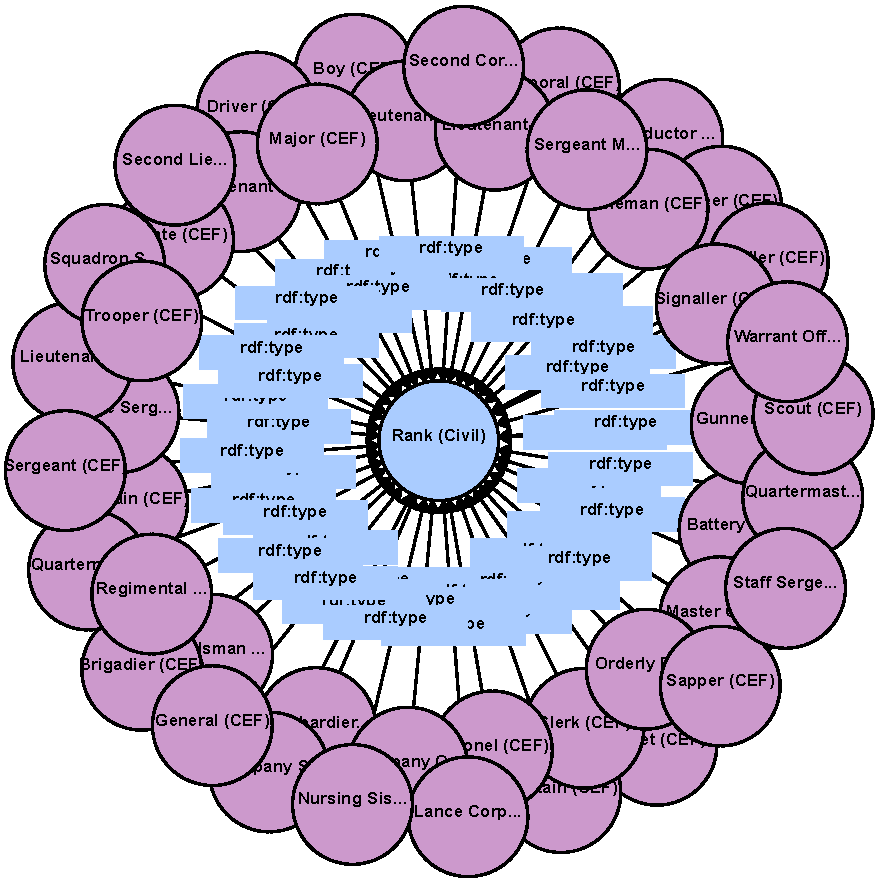
\includegraphics[width=8cm]{figures/code-list-visualized}
\caption{Visualization of a simple code list embedded in the Military Ontology v1.1 \cite{military_ontology}}
\label{fig:code-list-visualized}
%\vspace{-2mm}
\end{figure}

%There exist two common approaches to publishing a code list: 1) 
Aside such ontology-embedded structures, 
%sometimes also called \emph{value sets} \cite{alanrector}, 
the term `code list' is used for certain stand-alone datasets. %modeled using the SKOS vocabulary \cite{DBLP:journals/corr/abs-1801-04479}. 
Stand-alone code lists are being used, among other, in connection with government data %fiscal data where they have been defined as lists of values in a predefined set that can be used in metadata and that help metadata creators in selecting from a set of descriptors, thereby enhancing consistency and helping to avoid errors 
\cite{guide_code_list}, and modeled with the help of
%While some studies address the representation of code lists within specific domains using 
the SKOS vocabulary \cite{miles2009skos}. 
A typical case, applied, e.g., in fiscal open budget data \cite{DBLP:conf/smap/FilippidisKKIB16}, is the association of code lists with dimension properties of a multi-dimensional dataset conforming to the Data Cube\footnote{\url{https://www.w3.org/TR/vocab-data-cube/}} vocabulary \cite{obeu_dcv}.

While the structural patterns and lexical conventions of embedded vs.~stand-alone code lists differ, it seems worthwhile not only to analyze embedded code lists but also to expose them as independent resources, augmented with features that are common for stand-alone code lists. 

%we are unaware of any prior research that would systematically retrieve, extract and document \emph{code lists embedded in ontologies} in order to facilitate their reuse even across the detailed domains.
%focus on the usage of code lists across domains while also taking into account both mentioned code list specification modes.

%Both can be characterized by the typical structural (and sometimes also lexical) patterns, which could be expressed as SPARQL queries to be used to query vocabulary catalog endpoints and individual knowledge graphs. 

The most tangible contribution of our research is a collection of \emph{SPARQL queries} performing the extraction of embedded code lists from ontologies, currently from the Linked Open Vocabularies knowledge base aka LOV \cite{DBLP:journals/semweb/VandenbusscheAP17}, and a \emph{web application} (named Code List Analyzer) that allows to inspect the results. 
%Additional SPARQL queries can then be applied to a knowledge graph (we so far experimented with DBpedia) that would also contain code lists embedded in it.

%For the embedded code lists, we quantify their degree of adoption in comparison to the usage of their respective properties.

Given a broader perspective, we analyze embedded code lists from three different angles:
\begin{enumerate}
    \item As sets of RDF resources following some \emph{graph pattern} in the ontology, common for all of its members.
    \item As sets of \emph{ontological universals}. We hypothesize (and the subsequent analysis described in this paper confirmed) that the codes of embedded code lists can pre-dominantly be characterized as ontological universals, i.e., generic concepts that can be instantiated (even if the instantiation cannot happen due to their incidental syntactic encoding by individuals), in contrast to particulars, which cannot have instances (under any circumstances). For this reason, we will discuss in more detail -- as a contextual framing rather than in direct connection to the empirical research presented as the core contribution of the paper -- how concepts can be represented using RDF/OWL.
    \item As sets of \emph{syntactic individuals}. We thus, beyond extracting code lists using the graph context, also carry out an exhaustive examination of all syntactic individuals present in LOV ontologies, and attempt to characterize their role, which can also be different than that of code list codes.
\end{enumerate}

The remaining parts of this paper are organized as follows. 
%In Section 2 we review three structural parts of the semantic web knowledge representation: ontology schemas, code lists, and knowledge graphs, at a general level.  
In Section \ref{s:codelist-def} we start from an authoritative definition of code list from EU public service guidelines as well as from past research on OWL patterns, and attempt to derive from both a new formulation of versatile patterns characterizing embedded code lists in ontologies. 
In Section \ref{s:codelistanalyzer} we present an operational set of SPARQL queries based on those patterns, employed for detection and extraction embedded code lists, the enabling tool (Code List Analyzer), and the results achieved when applying this inventory on the LOV ontology collection.
Section \ref{s:skos_codelist_collecting} explains how the extracted code lists are `SKOSified' for better coherence and interoperability.
In Section \ref{s:repr} we first demonstrate the dominant nature of embedded codes as ontological universals, and, consequently, discuss three alternatives of representing universals (or, concepts) on the semantic web.
Section \ref{s:analysis_code_list_modeling_practice} describes a bottom-up analysis complementary to that from Section \ref{s:codelistanalyzer}; it starts from the set of all individuals inside all vocabularies, gradually partitioning their space by distinctive features, and, eventually, mapping these features to patterns from Section \ref{s:codelist-def}.
Section \ref{s:discussion} consists in a discussion of both quantitative and qualitative results from the previous analysis.
Section \ref{s:related} provides a comparison with related research.
Finally, Section \ref{s:conclusion} wraps up the paper.
%and outlines the directions for future work.
\section{Candidate code list patterns in RDF / OWL}
\label{s:codelist-def}

The notion of code list does not formally belong to the central ones in the semantic web: it does not appear, at least not under such a calling, anywhere in the core W3C recommendations (e.g., for RDF, OWL or SPARQL). 
Therefore, we decided to depart from the definition formulated in a highly authoritative document created in a specific corner of the semantic web field: the EU-endorsed \emph{Guidelines for the Use of Code Lists} \cite{guide_code_list} designed for  \emph{metadata management in public administration}; while RDF is considered as a possible technology for code list representation, it does not have an exclusive nor dominant position there. 
The purpose of this section is then to project the retrieved definition to the representation space of OWL ontologies (and, comparatively, instance-level RDF knowledge graphs) as our target in this paper.

Having said that, we however acknowledged a W3C note addressing a topic very similar to our notion of code list while not using this term: A.~Rector's treatment of `Representing Specified Values', from 2005 \cite{alanrector}. 
We will align our analysis with it, though arriving at slightly different engineering choices due to both the development of the semantic web landscape in the meantime and to the difference in focus: primarily inference-heavy ontologies in Rector's case, and mostly lightweight linked data vocabularies in our case, the latter assuming straightforward assignment of values to properties unconstrained by many ontological commitments in the Tbox.

The guidelines document \cite{guide_code_list}, developed under the EU SEMICS Action (addressing semantic interoperability), defines code lists as ``lists of \emph{values} in a \emph{predefined set} that can be used in metadata and that help metadata creators in \emph{selecting} from a set of descriptors, thereby enhancing consistency and helping to avoid errors'' (p.~3, italics purposefully added for notions that are pivotal for our purpose). 

\subsection{Syntactic status of codes for embedded code lists}
\label{ss:def_type}
Let us first interpret the notion of `value' from the above definition.
In the context of ontologies and other RDF graphs, we normally speak about \emph{values} in reference to \emph{properties} to which these values are assigned.
For ontologies (and knowledge graphs) to remain within the tractable OWL DL expressiveness fragment, such values can be either:
\begin{enumerate}
    \item Syntactic \emph{individuals}. 
    Individuals can be assigned to (object) properties entirely freely, under the open world assumption.
    The use of individuals is proposed in A.~Rector's Pattern 1, called \emph{value sets} \cite{alanrector}.
    Aside mere sets of individuals (usable as values of a property) Rector also includes three further elements of the pattern: first, a \emph{class} to which the instances belong as its \emph{enumeration} (through an \emph{owl:oneOf} axiom); second, the declaration of the individuals being pairwise different (through an \emph{owl:allDifferent} axiom); and third, \emph{value restrictions} (in description logic terms, existential restriction to a singleton nominal) on the property, which define each one derived class respective to the particular value.
    He demonstrates the pattern on the health status value \texttt{Good\_health\_value}, which is used to define a class \texttt{Healthy\_Person} via the property \texttt{has\_health\_status}. \\
    As downsides of the pattern, Rector mentions the impossibility to further sub-partition the values and the limited support of individuals by reasoners. The former limitation can however be overcome by employing a hierarchical partitioning suited for individuals (foremost, through \emph{skos:broader} and \emph{skos:narrower}), while the latter does not apply to nowaday's reasoners any longer.

    \item \emph{Classes}.
    Obviously, assigning classes via properties is a bit more complicated. 
    One possibility is to employ the \emph{punning}\footnote{\url{https://www.w3.org/TR/owl2-new-features/\#F12:\_Punning}} technique, i.e., interpreting the resource as an  individual merely having the same IRI as the corresponding class. 
    Since punning had not been allowed in OWL when A.~Rector wrote his note \cite{alanrector}, he designed a class-based pattern (Pattern 2), called \emph{value partition}, as relying on a (normal) existential restriction. In the example for this pattern, the health status value \texttt{Good\_health\_value} is therefore a class, and as such, it is not assigned to a person (\textt{John}) directly but through its instance \texttt{Johns\_Health} (or, alternatively, via an anonymous instance).\footnote{The instance is not materialized in this variant, but the assignment itself is done using an existential restriction: $\texttt{John} \in \exists \; \; \texttt{has\_health\_status} \; . \; \texttt{Good\_health\_value}$. We would not find such a method of assigning values much relevant when talking about code lists; in any case, it does not make any difference at the level of the ontology itself.}
    Other additional axioms are analogous to Pattern 1 but tailored to classes: there is a common \emph{superclass} of all values, and it is defined as their \emph{disjoint union}.
    
    \item \emph{Literals} (data values).
    Literals can also be easily assigned to (datatype) properties.
    A custom datatype could be defined to hold an enumerated list of values (as Rector mentioned in the preamble of his note), however, this is not a common practice in ontologies.
\end{enumerate}

Of the three possibilities of building the `predefined sets' \cite{guide_code_list}, we will immediately rule out the \emph{literals}.
Foremost, we do not normally find them in ontologies in the form of custom data types.
Second, more generally, the role of literals on the semantic web is primarily in the interaction with human users. 
While textual values may play the role of codelists in some RDF datasets, the fact that they are not globally unique identifiers (as IRIs) significantly compromises their machine-based interoperability.

Sets of \emph{classes}, if embedded in the form of Rector's value partition pattern, can surely be interpreted as code lists.
Merely as an engineering choice, we decided not to include them in our study, because
\begin{itemize}
    \item the pattern is not frequently used in linked data vocabularies (it is possibly more common, e.g., for some Bioportal\footnote{\url{https://bioportal.bioontology.org/}} ontologies, which tend to be more richly axiomatized)
    \item our ultimate goal is to expose the code lists as stand-alone SKOS structures; this would however require a `meta-modeling' transformation of `codes' from classes to individuals (instances of \emph{skos:Concept}), which is possible but would add a level of complexity to the process.
\end{itemize}

Therefore, for our purposes, we will only consider embedded code lists as sets of \emph{syntactic individuals} present in ontologies.
As regards the additional axioms of Rector's Pattern 1, we do not consider any of them (\emph{owl:oneOf}, \emph{owl:allDifferent} nor the value restriction) as necessary, as such strong ontological commitment is nowadays rather discouraged for linked data vocabularies. 
The fact that the values are distinct and exhaustively enumerated might be actually implicit but obvious to the user of the ontology, and the values are meant to be just assigned to dataset instances rather than used for defining a class.

\subsection{Graph patterns for capturing code lists}
\label{ss:def_patt}

In the RDF representation, a set of individuals can be glued together by several pattern techniques, most notably:
\begin{itemize}
    \item (\textbf{T1}) by being instances of a common class, i.e., appearing as subject in triples with predicate \emph{rdf:type} and the object being this class
    \item (\textbf{T2})  by appearing as objects in triples with the same predicate, and possibly also subject
    \item (\textbf{T3}) by appearing as subjects in triples with the same predicate (other than \emph{rdf:type}), and possibly also object.
\end{itemize}
Although the previous subsection only talked about code lists embedded in ontologies, it should be mentioned that \emph{sets} of `sibling' individuals might be identified both in ontologies (concept-level knowledge bases) and in  knowledge graphs (instance-level knowledge bases), in principle.
The problem of \emph{instance-level} graphs is however their usually large size and open nature, which discourages from viewing such `sibling sets' as intentionally \emph{pre-defined} code lists.
Also the target mentioned in the definition from the guidelines \cite{guide_code_list}, `enhancing consistency' (between independently created resources that reuse the given code list), have better chance to be achieved via \emph{ontologies}, since they are more likely to be widely reused than most instance-level knowledge graphs (even if especially encyclopaedic KGs, such as Wikidata or DBpedia, do enjoy extensive reuse by reference).

Looking at \emph{ontologies}, we see that individuals only appear in some of them.
Their small number, never mind the mere nature of ontologies as compact artifacts, indicates that the introduction to individuals to ontologies may satisfy the assumption of intentionally \emph{predefined} sets of values from the Guidelines \cite{guide_code_list}. 
Considering the concept-level nature of ontologies, we can conjecture a limited number of motivations why individuals would enter this company:\footnote{Note that A. Rector's Pattern 1 \cite{alanrector} encompasses three of the motivations, \textbf{M1}, \textbf{M2} and \textbf{M3}. However, in real cases the motivations could possibly arise even independently of each other.}
\begin{itemize}
    \item (\textbf{M1}) In order to specify the \emph{allowed values} that can be \emph{assigned to a property}.
    \item (\textbf{M2}) In order to \emph{define a class} as an \emph{enumeration} of individuals (one-of restriction). 
    \item (\textbf{M3})  In order to \emph{define a class} through a \emph{property-value pair} (value restriction, i.e. existential restriction with a singleton class in its filler)  
    \item (\textbf{M4}) In order to explain the meaning of a class through its \emph{example instances}.
\end{itemize}
Intuitively, \textbf{M1}  is coherent with the notion of code list, see the formulation ``\emph{selecting from a set} of descriptors'' in the definition from the guidelines \cite{guide_code_list}, since the property with the value together form a descriptor to be selected.
Also  \textbf{M2} to some degree fits the notion of code list: the set of values is \emph{closed}.
However, the `selection' (of a value to a property) is not explicit.
\textbf{M3}  is less relevant, since it only assumes a single, possibly isolated, individual, that allows to define a single class.
Finally, \textbf{M4}  is clearly beyond the notion of code list, since example instances are by no means `pre-defined'.

We can now compare these motivations with the three graph pattern techniques of grouping individuals above. 

We immediately see that \textbf{T1} -- instantiation of a common class -- plays an important role in most of the motivations.
For \textbf{M1}, the link between a property and a set of individuals is most straightforwardly expressed by introducing a class over-arching these individuals and making this class the range of the property (or possibly the filler of local universal restrictions).
\textbf{M2} and \textbf{M4} introduce such a class inherently.
Thus only \textbf{M3} does not necessitate the introduction of a class (and a \emph{set} of individuals instantiating it) -- but it is possible that in order to define a \emph{set of classes} of a similar kind, instances (value restriction fillers) belonging to a common class would come into play.\footnote{As an example, though a merely educative one, consider the well-known \emph{Pizzas} ontology, \url{https://protege.stanford.edu/ontologies/pizza/pizza.owl} used to illustrate the common caveats of OWL ontology modeling \cite{DBLP:conf/ekaw/RectorDHRKSWW04}. There classes of pizzas such as \texttt{RealItalianPizza} or \texttt{American} are defined through a value restriction on property \texttt{hasCountryOfOrigin}, with fillers such as \texttt{Italy} or \texttt{America}, all being instances of class \texttt{Country}.}

Technique \textbf{T2} -- individuals as values of the same property -- is only expressed indirectly in the ontology itself in the case of motivation \textbf{M1}, namely, via a range axiom, or local restriction/s, whose filler is the class of those individuals,\footnote{The filler also could be the enumeration of values instead of a named class, such a practice would however be very usual in the context of using a range axiom in linked data vocabularies.} see the previous paragraph. 
(Obviously, the relation between the individuals and properti/es is foreseen in the datasets referring to the given ontology.)
Similarly, for \textbf{M3} the property appears in the value restriction.
The remaining motivations, \textbf{M2} and \textbf{M4}, do not consider an `assignment' property associated with them.
As regards the grouping of individuals in the object of triples sharing  \emph{both the predicate and subject}, it is completely irrelevant for our case, since in \textbf{M1} the subject of the triples is not considered at all,\footnote{When specifically considering code lists, by our experience it is rather uncommon for different conceptual types of subject entities to be described by the same code list property.} and in \textbf{M3} each code defines a different class (each presumably instantiating a disjoint set of individuals in datasets).

Finally, technique \textbf{T3} -- individuals as subjects used with the same property, and possibly the same object -- is not inherently part of any of the motivations.
Note that to satisfy the assumption of the code list being `pre-defined', we need a property whose semantics would suggest that the identity of its object determines a stable collection of resources that can appear as its subject.
In this respect, we deem the property \emph{skos:inScheme} as highly relevant.
The situation of a set of individuals being concepts (instances of \emph{skos:Concept}) belonging to the same SKOS scheme (i.e., linked through \emph{skos:inScheme} to a particular instance of \emph{skos:ConceptScheme}) is analogous to the situation of a set of individuals being instances of a particular domain-specific class in the ontology.

\subsection{Summary}
Based on the considerations from this section, we may characterize the candidate structures for code lists in OWL ontologies as follows: 
\begin{itemize}
    \item They are NECESSARILY sets of syntactic \emph{individuals}, i.e. neither literals nor classes (cf. Section~\ref{ss:def_type}).\footnote{We would like to recall that we consider this merely as an engineering decision, eliminating literals due to their problematic machine-processability and classes due to the subsequent reliance on OWL restrictions and need of far-reaching representational transformations. Follow-up research will possibly consider these, especially the classes (`value partitions' in A. Rector's style).} 
    \item The individuals are PREFERABLY \emph{instances of a common class} from the ontology (cf. technique \textbf{T1} in Section~\ref{ss:def_patt}).
    This class is OPTIONALLY in the range of at least one \emph{property}.
    \item The individuals are PREFERABLY instances of \emph{skos:Concept}, and linked by the \emph{skos:inScheme} property to the same \emph{skos:ConceptScheme} instance (cf. technique \textbf{T3} in Section~\ref{ss:def_patt}).
%    \item The individuals are OPTIONALLY declared as different individuals (through \emph{owl:differentFrom} or \emph{owl:allDifferent}).
%    \item The individuals are OPTIONALLY instances of a class \emph{enumerating them} (through \emph{owl:oneOf}).
\end{itemize}
This (`fuzzy') pattern will be reflected in the subsequent formulation of SPARQL queries aiming to retrieve the relevant structures from real vocabularies (Section~\ref{s:codelistanalyzer}).
Note that the technique \textbf{T2} is only included as optional, as it is redundant for code list extraction with respect to \textbf{T1} (i.e., ``if there is an assignment property in the ontology, there is also a filler class''). 
%However, we will take the assignment property into consideration in the bottom-up analysis covering all individuals (Section~\ref{s:analysis_code_list_modeling_practice}).
%\input{sections/02-structural-parts}
\section{Candidate code list exploration} 
\label{s:codelistanalyzer}

We describe here a proof-of-concept experiment, which involves query-based exploration of candidate code lists in the LOV knowledge base, in which we can find the description of RDFS vocabularies and OWL ontologies defined for and used by datasets on the Linked Data Cloud.

The goal of this part of our research has been to create and apply a collection of SPARQL queries that can be used in the process of exploring code lists in LOV. % and other knowledge bases as well. %Another specific goal was to identify the coverage of knowledge instances with respect to their abstract concepts. 

\subsection{Query sequence for candidate code list exploration}
The detection and extraction of code lists in a vocabulary consist of several steps and five main exploratory queries. The exact parameterized SPARQL queries labeled Q1 through Q5 can also be found on the mentioned GitHub repository homepage.

For reproducibility purposes, the steps of this experiment are summarized as follows:

\begin{enumerate}
    \item Make a list of vocabularies that might contain code lists, sorted by the number of included individuals and classes.

    \item In each vocabulary, find all classes and count the number of their instances.% and subclasses.

    \item For each class with at least one instance, find all its instances (individuals) and check if these instances are connected to \emph{skos:Concept} (which is known to be used for codes in code lists).

    \item Query for direct relationships between these instances and use this information to visualize the candidate code list (see e.g. Figure \ref{fig:code-list-visualized})

    \item Query for the instance-instance relationships (assignment properties) that exist in each vocabulary, including the total number of instances on both sides of the relationships (this helps to check if we missed any codes).

\end{enumerate}

Using this procedure, we collected all candidate code lists for further review. If a result proves to be a code list but does not use \emph{skos:Concept}, we enhance it by connecting the collected codes with \emph{skos:Concept}, and their class with \emph{skos:ConceptScheme} (using SPARQL UPDATE, see Code listing \ref{lst:sparql6}). The enhanced data are then compiled into one knowledge base, which provides simpler and more straightforward access to the code lists thanks to SKOS.



Note that none of the queries is to be understood as a strict definition of what should be a code list.
Instead, the queries assemble collections of results that can be independently inspected and gradually produce a code list knowledge base potentially useful for the community (without guaranteeing that every single element would fully satisfy a rigorous or common-sense concept of what should a code list be).
The queries, especially, Q3 and Q4, are derived from the analysis presented in the previous section. 

\medskip
\medskip
\noindent\textbf{Q1: Identify the named graph IRIs of the target vocabularies}. This step retrieves a list of vocabulary IRIs and their names. In addition, we also query for the number of classes and class instances in each vocabulary.\footnote{Note that here we are using the \textit{GRAPH} keyword to determine the boundaries in which we count the classes and class instances for each vocabulary. This is thanks to the fact that LOV maintains each vocabulary in a separate graph. Another intuitive approach to get the same results is to use the \textit{rdfs:isDefinedBy} property. However, this approach is unreliable because not all vocabularies use this property to define their terms. To make it reliable, we would have to enhance the data by adding it to all the terms in each vocabulary. This can be done using
%keyword some vocabularies are not listed here even though they include class instances. This is because this query assumes the classes have the property \textit{rdfs:isDefinedBy} so that their number can be counted for each vocabulary. This can be fixed by 
query Q0 (described in our GitHub repository README) before running query Q1. However, this would require setting up a custom endpoint with SPARQL UPDATE feature enabled. Also, we only retrieve English labels or labels with no specified language.} In LOV, the total number of vocabularies having at least one class instance is 271 (out of all 818 vocabularies). A part of the results for this query is displayed in Table \ref{tab:q1-results}, which lists the top vocabularies with the highest number of class instances. The number of classes and instances indicates the probability of code lists existing in each vocabulary and helps to set the priority for analyzing each vocabulary. Vocabularies that have a low number of classes and instances will probably be less likely to include code lists. %This way, the analysis procedure would find the majority of code lists in the targeted knowledge base sooner.

\begin{lstlisting}[captionpos=b, caption=Q1 -- Query to get a list of vocabularies with class count and class instance count,label=lst:sparql1,basicstyle=\small\ttfamily,frame=single]
SELECT DISTINCT ?v
 (GROUP_CONCAT(DISTINCT ?vp;separator="|") AS ?vps)
 (GROUP_CONCAT(DISTINCT ?vl;separator="|") AS ?vls)     
 (COUNT (DISTINCT ?c) AS ?nc)
 (COUNT (DISTINCT ?i) AS ?ni)
WHERE {
  ?v a voaf:Vocabulary .
  OPTIONAL { ?v vann:preferredNamespacePrefix ?vp }
  OPTIONAL {
    VALUES ?vlp { rdfs:label skos:prefLabel
                  dc:title dcterms:title }
    ?v ?vlp ?vl .
    FILTER(LANGMATCHES(LANG(?vl), 'en') ||
           LANGMATCHES(LANG(?vl), '')) }
  OPTIONAL {
    GRAPH ?v {
      VALUES ?class { owl:Class rdfs:Class } .
      ?c a ?class . OPTIONAL { ?i a ?c } } }
} GROUP BY ?v ORDER BY DESC(?ni)
\end{lstlisting}

\begin{table}[h]
\footnotesize
\centering
\begin{tabular}{|l|l|r|r|}
\hline
\textbf{\texttt{?vps}} & \textbf{\texttt{?vls}}                      & \textbf{\texttt{?nc}} & \textbf{\texttt{?ni}} \\ \hline
\hline
\textbf{Prefix} & \textbf{Label}                                                                 & \textbf{Class} & \textbf{Inst.} \\ \hline
losp       & Linked open specialities RF                                                                     & 6    & 2\,009 \\ \hline
cfp        & Climate and Forecast standard                                                                   & 48   & 1\,972 \\ \hline
cff        & Climate and Forecast features                                                                   & 48   & 1\,666 \\ \hline
oum        & Ontology of units of Measure                                                                    & 1\,078 & 1\,601 \\ \hline
ifc        & IFC4\_ADD1                                                                                      & 1\,395 & 1\,155 \\ \hline
cwrc       & The CWRC Ontology                                                                               & 124  & 823  \\ \hline
gn         & The Geonames ontology                                                                           & 7    & 699  \\ \hline
ids        & IDS Information Model                                                                           & 290  & 675  \\ \hline
mil        & The Muninn Military Ontology                                                                    & 142  & 667  \\ \hline
semsur     & SemSur, Version 2.0                                                                             & 3\,890 & 329  \\ \hline
common     & The Delivery Context Ontology                                                                   & 150  & 314  \\ \hline
geop       & Geopolitical Ontology                                                                           & 11   & 312  \\ \hline
uniprot    & Uniprot Core Ontology                                                                           & 252  & 312  \\ \hline
obo        & Ontology for Biomedical Investi.                                                                & 5\,374 & 296  \\ \hline
ceo        & CEO: Consumer Electronics Ont.                                                                  & 49   & 285  \\ \hline
lexinfo    & LexInfo                                                                                         & 279  & 275  \\ \hline
odrl       & ODRL Version 2.2                                                                                & 45   & 239  \\ \hline
aos        & Sex, Genders, Preferences and                                                                   & 39   & 237  \\ \hline
topo       & An ontology for describing terri.                                                               & 52   & 226  \\ \hline
jup        & Ontology of Building Accessib.                                                                  & 48   & 206  \\ \hline
geosp      & GeoSpecies Ontology                                                                             & 86   & 204  \\ \hline
vin        & Wine Ontology                                                                                   & 101  & 161  \\ \hline
cbo        & Comic Book Ontology                                                                             & 68   & 138  \\ \hline
sw-quality & SQuAP Ontology                                                                                  & 153  & 135  \\ \hline
%uby        & ubyCat.owl                                                                                      & 53   & 134  \\ \hline
%pmovn      & Predicate Model for Ontologies                                                                  & 53   & 133  \\ \hline
%modsci     & ModSci, Modern Science Ontology                                                                 & 244  & 130  \\ \hline
%scoro      & Scholarly Contributions and Roles                                                               & 20   & 125  \\ \hline
%schema     & Schema.org vocabulary                                                                           & 625  & 124  \\ \hline
%chord      & The Chord Ontology                                                                              & 9    & 108  \\ \hline
%turismo    & Ontology of Tourist for Saragossa town hall.                                                    & 51   & 102  \\ \hline
%rsctx      & Recommender System Context                                                                      & 52   & 91   \\ \hline
%ddesc      & Denotative Description Ontology (ArCo network)                                                  & 66   & 91   \\ \hline
%citof      & CiTOFunction                                                                                    & 6    & 84   \\ \hline
%sh         & W3C Shapes Constraint Language (SHACL) Vocabulary                                               & 40   & 79   \\ \hline
%s4watr     & SAREF extension for water                                                                       & 72   & 78   \\ \hline
%gold       & General Ontology for Linguistic Description                                                     & 502  & 76   \\ \hline
%voag       & Vocabulary Of Attribution and Governance                                                        & 65   & 76   \\ \hline
%iot-tta    & Ontology for Internet of Things Technologies, Tools, and Applications                           & 152  & 76   \\ \hline
%pext       & Proton Ontology                                                                                 & 488  & 72   \\ \hline
%mv         & MobiVoc: Open Mobility Vocabulary                                                               & 38   & 68   \\ \hline
%sdmx-code  & SDMX Code                                                                                       & 9    & 66   
\end{tabular}
\caption{Q1 sample result (formatted)} \label{tab:q1-results}.
%\vspace{-6mm}
\end{table}

\medskip
\noindent\textbf{Q2: Get a list of instantiated classes with the number of their instances}. From a vocabulary (whose IRI is the parameter of this query), we retrieve classes that have at least one instance. The number of instances indicates the possible size of the candidate code list. We assume that the code list members could be referenced by other entities; we thus also query for the incoming property edge (assignment property) and its domain entity. This means that the class can be the value of \textit{rdfs:range} of the assignment property. We can observe in the query results that not many candidate code lists have an assignment property. % and we presume that these instances are probably not meant to be code lists. They could be just exemplary instances added to the ontology for the illustration of the classes, or because they are considered important in the domain. These cases should be further analyzed based on the meanings of these instances. 
Result examples for query Q2 are displayed in Table \ref{tab:q2-results}.

\begin{lstlisting}[captionpos=b, caption=Q2 -- Query to get the number of instances of each class in an ontology with their range properties and domain classes,label=lst:sparql2,basicstyle=\small\ttfamily,frame=single]
SELECT ?d ?p ?c (COUNT(DISTINCT ?i) AS ?ni)
FROM <${vocab}>
WHERE {
  VALUES ?class { rdfs:Class owl:Class }
  ?c a ?class .
  ?i a ?c .
  OPTIONAL { 
    ?p rdfs:range ?c . 
    OPTIONAL { ?p rdfs:domain ?d }
  }
} GROUP BY ?d ?p ?c ORDER BY DESC(?ni)
\end{lstlisting}

\begin{table}[ht]
\footnotesize
\centering
\begin{tabular}{|l|l|l|r|}
\hline
\textbf{\texttt{?d}}      & \textbf{\texttt{?p}} & \textbf{\texttt{?c}} & \textbf{\texttt{?ni}} \\ \hline
\hline
\textbf{Domain}  & \textbf{Property} & \textbf{Code list} & \textbf{Codes} \\ \hline
mil:PostToUnit   & mil:toUnit        & mil:MilitaryRank           & 605              \\ \hline
foaf:Person      & mil:heldRank      & mil:MilitaryRank           & 605              \\ \hline
org:Organizat.   & mil:rankOf        & mil:MilitaryRank           & 605              \\ \hline
                 &                   & mil:Rank                   & 45               \\ \hline
                 &                   & mil:Soldier                & 34               \\ \hline
                 &                   & mil:MilitaryTrade          & 18               \\ \hline
                 &                   & mil:MilitaryAppo.          & 14               \\ \hline
                 &                   & mil:ArmsType               & 8                \\ \hline
                 &                   & mil:BattleSpace            & 5                \\ \hline
                 &                   & mil:Non-Combat.            & 2                \\ \hline
                 &                   & mil:Role                   & 1                \\ \hline
\end{tabular}
\caption{Q2 sample result for the Military ontology (formatted)} \label{tab:q2-results}
%\vspace{-6mm}
\end{table}

\medskip
\medskip
\medskip
\noindent\textbf{Q3: Get a list of candidate code list members}. This query gives us an overview of all members of the candidate code lists. Here, we retrieve the instances %and subclasses 
of each class in each vocabulary. The vocabulary and the class are the two parameters of this query. The query results are not yet considered code lists but are understood as a mixture of class instances found inside each ontology. In this query, we also look for whether a code list member is tagged with \emph{skos:Concept}. The fact that the class instances are annotated with \emph{skos:Concept} makes it easier to reference them from other knowledge graphs; thanks to \emph{skos:Concept}, the code list can be effectively extracted as a standalone resource (described in Section \ref{s:skos_codelist_collecting}). Examples of results for this query are displayed in Table \ref{tab:q3-results}.

\begin{lstlisting}[captionpos=b, caption=Q3 -- Query to get a list of candidate code list members and whether they are tagged with \textit{skos:Concept} and \textit{skos:inScheme},label=lst:sparql3,basicstyle=\small\ttfamily,frame=single]
SELECT DISTINCT ?i (BOUND(?sc) AS ?bsc)
                   (BOUND(?scs) AS ?bscs)
FROM <${vocab}>
WHERE {
  ?i a <${class}> .
  OPTIONAL {
    BIND(skos:Concept AS ?sc) .
    ?i a ?sc .
  }
  OPTIONAL {
    ?i skos:inScheme ?scs .
    ?scs a skos:ConceptScheme .
  }
}
\end{lstlisting}

\begin{table}[h]
\footnotesize
\centering
\begin{tabular}{|l|c|c|}
\hline
\textbf{\texttt{?i}}      & \textbf{\texttt{?bsc}} & \textbf{\texttt{?bscs}}      \\ \hline \hline
\textbf{Instance}         & \textbf{skos:Concept}  & \textbf{skos:inScheme}       \\ \hline
mil:1AIFRankCaptain       & Yes                    & No                           \\ \hline
mil:1AIFRankGunner        & Yes                    & No                           \\ \hline
mil:1AIFRankPrivate       & Yes                    & No                           \\ \hline
mil:1AIFRankEngineer      & Yes                    & No                           \\ \hline
mil:1AIFRankNurse         & Yes                    & No                           \\ \hline
mil:1AIFRankCorporal      & Yes                    & No                           \\ \hline
mil:1AIFRankTrooper       & Yes                    & No                           \\ \hline
mil:1AIFRankChaplain      & Yes                    & No                           \\ \hline
mil:1AIFRankSergeant      & Yes                    & No                           \\ \hline
mil:1AIFRankDriver        & Yes                    & No                           \\ \hline
mil:1AIFRankMajor         & Yes                    & No                           \\ \hline
mil:1AIFRankSapper        & Yes                    & No                           \\ \hline
mil:1AIFRankSignaller     & Yes                    & No                           \\ \hline
mil:1AIFRankLieutenant    & Yes                    & No                           \\ \hline
\end{tabular}
\caption{Q3 sample result for class \textit{mil:Soldier} in the Military ontology (formatted)} \label{tab:q3-results}
%\vspace{-6mm}
\end{table}

\medskip
\noindent\textbf{Q4: In each candidate code list, get all code list members' data including the relationships between them}. This step is to construct and visualize the candidate code list. For this, we need to query all information about the code list members. As we have mentioned before, a code list can simply have a flat structure, but it can also form a shallow hierarchy via properties such as \textit{skos:broader} or \textit{rdfs:subClassOf}\footnote{\label{note:owlSubClass}The properties \textit{owl:subClassOf} and \textit{owl:subClass} do not exist in the OWL specification, they are however used in the Military ontology. This is probably a mistake made by the authors. We understand that these properties should be \textit{skos:broader} or \textit{rdfs:subClassOf} according to the meanings of the codes, similarly in the case of \textit{org:rankEquivalentTo}, \textit{org:rankSeniorToTransitive}, \textit{org:rankJuniorToTransitive} in Table \ref{tab:q5-results} and some others}. The query results in Table 4 show an example of this particular finding in the Military ontology. To show that this approach can be applied to any vocabulary, Figure \ref{fig:code-list-with-hierarchy} shows the visualization of a code list structure about weekdays from the GoodRelations ontology.


\begin{lstlisting}[captionpos=b, caption=Q4 -- Query to get candidate code list structure,label=lst:sparql4,basicstyle=\small\ttfamily,frame=single]
SELECT DISTINCT ?cn ?i1 ?i1n ?p ?i2 ?i2n
FROM <${vocab}> WHERE {
  ?i1 a <${class}> .
  VALUES ?lp { rdfs:label skos:prefLabel
               dc:title dcterms:title }
  OPTIONAL {
    <${class}> ?lp ?cn . 
    FILTER(LANGMATCHES(LANG(?cn), 'en'))
  }
  OPTIONAL {
    ?i1 ?lp ?i1n . 
    FILTER(LANGMATCHES(LANG(?i1n), 'en'))
  }
  OPTIONAL {
    ?i2 a <${class}> . ?i1 ?p ?i2 .
    OPTIONAL { 
      ?i2 ?lp ?i2n . 
      FILTER(LANGMATCHES(LANG(?i2n), 'en'))
    }
  }
} ORDER BY ?i1
\end{lstlisting}

\begin{table}[ht]
\footnotesize
\centering
\begin{tabular}{|l|l|l|}
\hline
\textbf{\texttt{?i1}}       & \textbf{\texttt{?p}}                     & \textbf{\texttt{?i2}}       \\ \hline \hline
\textbf{Code 1}             & \textbf{Relationship}                    & \textbf{Code 2}             \\ \hline
2nd Corporal                &                                          &                             \\ \hline
2nd Lieutenant              & owl:subClassOf\cref{note:owlSubClass}    & Lieutenant                  \\ \hline
Able Seaman                 &                                          &                             \\ \hline
Air Mechanic                &                                          &                             \\ \hline
Air Mechanic Class I        & owl:subClassOf\cref{note:owlSubClass}    & Air Mechanic                \\ \hline
Air Mechanic Class II       & owl:subClassOf\cref{note:owlSubClass}    & Air Mechanic                \\ \hline
Lieutenant                  &                                          &                             \\ \hline
Sapper                      &                                          &                             \\ \hline
Sergeant                    &                                          &                             \\ \hline
Sergeant Major              &                                          &                             \\ \hline
Signaler                    &                                          &                             \\ \hline
Staff Sergeant              &                                          &                             \\ \hline
\end{tabular}
\caption{Q4 sample result for class \textit{mil:Soldier} in the Military ontology (formatted)} \label{tab:q4-results}
%\vspace{-6mm}
\end{table}

\medskip
\noindent\textbf{Q5: Get a list of distinct properties that connect two code list members}. Optionally, we can verify our results using an additional query that will retrieve all properties connecting the two code list members. Examples of the results for this query are shown in Table \ref{tab:q5-results} which includes the number of connected subjects and objects via a particular predicate.

\begin{lstlisting}[captionpos=b, caption=Q5 -- Query to get a list of properties that connect class instances (also shows the number of instances on both sides),label=lst:sparql5,basicstyle=\small\ttfamily,frame=single]
SELECT (COUNT(DISTINCT ?i1) AS ?ni1) ?p 
       (COUNT(DISTINCT ?i2) AS ?ni2)
FROM <${vocab}> WHERE {
  VALUES ?class { owl:Class rdfs:Class }
  ?c1 a ?class .
  ?c2 a ?class .
  ?i1 a ?c1 .
  ?i2 a ?c2 .
  ?i1 ?p ?i2 .
} GROUP BY ?p
\end{lstlisting}


\begin{table}[h]
\footnotesize
\centering
\begin{tabular}{|r|l|r|}
\hline
\textbf{\texttt{?ni1}}     & \textbf{\texttt{?p}}                  & \textbf{\texttt{?ni2}} \\ \hline \hline
\textbf{Subj. Codes}       & \textbf{Property}                     & \textbf{Obj. Codes}    \\ \hline
384                        & owl:subClass\cref{note:owlSubClass}   & 130                    \\ \hline
41                         & org:rankEquivalentTo*                 & 41                     \\ \hline
39                         & mil:rankOf                            & 5                      \\ \hline
36                         & org:rankJuniorToTransitive*           & 35                     \\ \hline
35                         & org:rankSeniorToTransitive*           & 36                     \\ \hline
33                         & skos:inScheme                         & 5                      \\ \hline
32                         & owl:subClassOf\cref{note:owlSubClass} & 27                     \\ \hline
1                          & owl:disjointWith                      & 1                      \\ \hline
1                          & skos:broader                          & 1                      \\ \hline
\end{tabular}
\footnotesize
\caption{Q5 results for the Military ontology (formatted)\\ \**\textit{these properties do not exist in the Core Organization ontology}} \label{tab:q5-results}
%\vspace{-6mm}
\end{table}


\begin{figure}[h]
\centering
%\captionsetup{justification=centering}
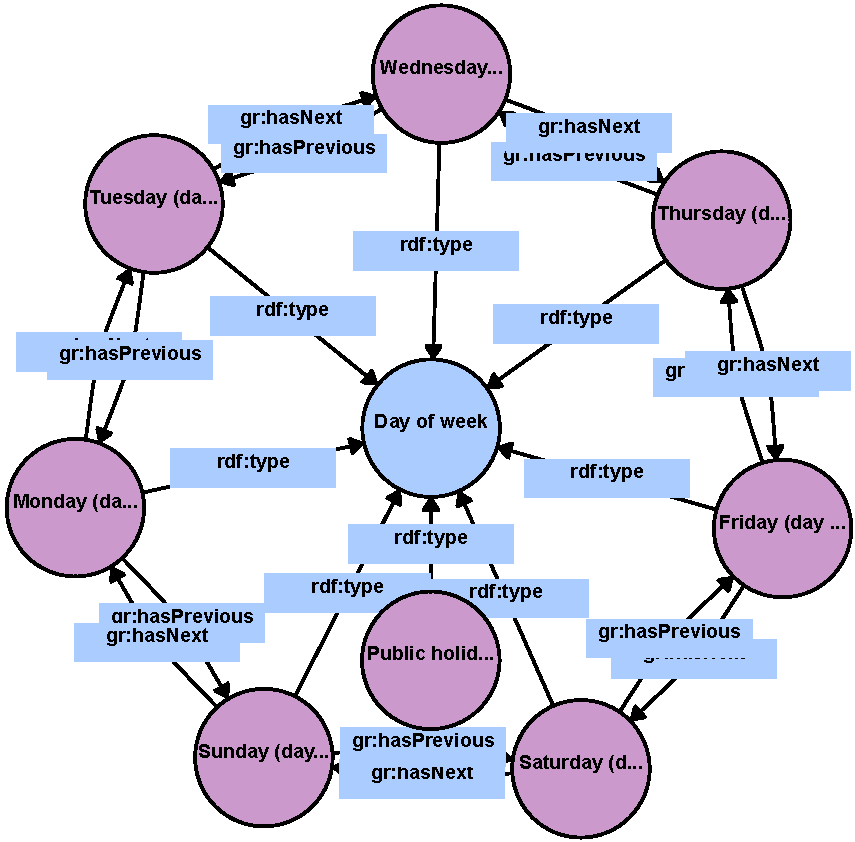
\includegraphics[width=8cm]{figures/code-list-days-of-week}
\caption{Visualization of a simple code list that forms a hierarchy in the GoodRelations vocabulary}
\label{fig:code-list-with-hierarchy}
%\vspace{-4mm}
\end{figure}

\subsection{Implementation: Code List Analyzer}

To make the process of browsing candidate code lists simpler, we have implemented a web application called Code List Analyzer, which uses these queries in our workflow to enable more comprehensive analysis and to provide empirical insight into the queried data.

The source code of our project is available on GitHub\footnote{\label{github-repo}\url{https://github.com/nvbach91/iga-hybrid}} under an open-source license. The web client Code List Analyzer is accessible online via the following link: \url{https://fcp.vse.cz/iga-hybrid}.

\subsection{Results}

The above sequence of SPARQL queries Q1 through Q5 is implemented in our Code List Analyzer tool and has been successfully executed on a total of 818 LOV vocabularies. % (that have at least one class instance). 
We have discovered in aggregation\footnote{\url{https://github.com/nvbach91/iga-hybrid/tree/master/aggregate} (includes scripts to reproduce the results)} that 567 vocabularies do not have any code lists embedded in them. %, probably because these vocabularies are small. 
In 251 of the processed vocabularies, there are structures embedded that resemble code lists. The total number of candidate code lists detected in these vocabularies is 1\,690 and the total number of candidate code list members is 21\,747.

The top vocabularies that have the highest number of candidate code lists and the top vocabularies that have the highest number of code list members along with their SKOS status are listed in Table \ref{tab:top-codes}. There are only 16 vocabularies that use SKOS to model the instances.

\begin{table}[h]
\footnotesize
\begin{tabular}{|l|r|l|}
\hline
\textbf{Vocab} & \textbf{CLists} & \textbf{SKOS} \\ \hline
*add1     & 206         & No   \\ \hline
common    & 79          & No   \\ \hline
obo       & 50          & No   \\ \hline
cfp       & 48          & No   \\ \hline
cff       & 47          & No   \\ \hline
lexinfo   & 41          & No   \\ \hline
vin       & 39          & No   \\ \hline
oum       & 38          & No   \\ \hline
ids       & 37          & Yes  \\ \hline
semsur    & 37          & No   \\ \hline
ceo       & 36          & No   \\ \hline
ontosec   & 31          & No   \\ \hline
modsci    & 31          & No   \\ \hline
iot-tta   & 27          & No   \\ \hline
geosp     & 24          & No   \\ \hline
aos       & 24          & No   \\ \hline
voag      & 22          & No   \\ \hline
gc        & 22          & No   \\ \hline
...       & ...         & ...   \\ \hline
%uby       & 20          & No   \\ \hline
%cwrc      & 19          & Yes  \\ \hline
%bevon     & 18          & No   \\ \hline
%fowl      & 18          & No   \\ \hline
%turismo   & 15          & No   \\ \hline
%qudt      & 14          & No   \\ \hline
%cbo       & 14          & No   \\ \hline
%topo      & 13          & Yes  \\ \hline
%ldr       & 13          & No   \\ \hline
%scoro     & 12          & No   \\ \hline
%maso      & 12          & No   \\ \hline
%security  & 12          & No   \\ \hline
%cdesc     & 12          & No   \\ \hline
%dk        & 12          & Yes  \\ \hline
%cwmo      & 11          & No   \\ \hline
%ocds      & 11          & No   \\ \hline
%sims      & 10          & No   \\ \hline
%s4watr    & 10          & No   \\ \hline
%bimerr-op & 10          & No   \\ \hline
%rsctx     & 10          & No   \\ \hline
%akt       & 9           & No   \\ \hline
%gr        & 9           & No   \\ \hline
%mil       & 9           & Yes  \\ \hline
%ddesc     & 9           & No   \\ \hline
\end{tabular}
\,
\begin{tabular}{|l|r|l|}
\hline
\textbf{Vocab} & \textbf{Codes} & \textbf{SKOS} \\ \hline
losp           & 2009 & No  \\ \hline
cfp            & 1974 & No  \\ \hline
oum            & 1852 & No  \\ \hline
cff            & 1668 & No  \\ \hline
*add1          & 1627 & No  \\ \hline
semsur         & 1158 & No  \\ \hline
cwrc           & 837  & Yes \\ \hline
mil            & 728  & Yes \\ \hline
ids            & 702  & Yes \\ \hline
gn             & 699  & No  \\ \hline
lexinfo        & 669  & No  \\ \hline
geosp          & 429  & No  \\ \hline
uniprot        & 372  & No  \\ \hline
odrl           & 369  & Yes \\ \hline
common         & 349  & No  \\ \hline
geop           & 312  & No  \\ \hline
obo            & 304  & No  \\ \hline
ceo            & 285  & No  \\ \hline
...            & ...  & ... \\ \hline
%aos            & 242  & No  \\ \hline
%topo           & 233  & Yes \\ \hline
%vin       & 39  & 161  & No  \\ \hline
%cbo       & 14  & 138  & No  \\ \hline
%uby       & 20  & 136  & No  \\ \hline
%*squap    & 4   & 135  & No  \\ \hline
%pmovn     & 6   & 133  & No  \\ \hline
%*modsci   & 31  & 130  & No  \\ \hline
%scoro     & 12  & 125  & No  \\ \hline
%chord     & 5   & 108  & No  \\ \hline
%turismo   & 15  & 102  & No  \\ \hline
%citof     & 5   & 94   & No  \\ \hline
%rsctx     & 10  & 91   & No  \\ \hline
%ddesc     & 9   & 91   & No  \\ \hline
%s4watr    & 10  & 78   & No  \\ \hline
%voag      & 22  & 77   & No  \\ \hline
%*iot-tta  & 27  & 76   & No  \\ \hline
%gold      & 1   & 76   & No  \\ \hline
%spfood    & 8   & 75   & No  \\ \hline
%pext      & 6   & 72   & No  \\ \hline
%mv        & 8   & 68   & No  \\ \hline
%sdmx-code & 7   & 66   & Yes \\ \hline
%nlon      & 5   & 65   & No  \\ \hline
%ontosec   & 31  & 63   & No  \\ \hline
%akt       & 9   & 62   & No  \\ \hline
\end{tabular}
\centering
%\captionsetup{justification=centering}
\caption{Top vocabularies with the highest number of embedded code lists and code list members} %(*ce: consumerelectronics, mv: mobivoc)}
\label{tab:top-codes} 
%\vspace{-6mm}
\end{table}

The number of vocabularies with at least one assignment property is 156. The remaining 662 vocabularies do not contain any assignment properties. The total number of candidate code lists with at least one assignment property is 782 and the total number of candidate code lists without assignment properties is 908.

\begin{table}[h]
\footnotesize
\centering
\begin{tabular}{|l|r|}
\hline
\textbf{Statistics}                                         & \textbf{Value} \\ \hline
Vocabularies                                                & 818            \\ \hline
Vocabularies using SKOS                                     & 16             \\ \hline
Vocabularies with candidate code lists                      & 251            \\ \hline
Vocabularies without candidate code lists                   & 567            \\ \hline
Vocabularies with codes                                     & 251            \\ \hline
Vocabularies with assignment properties                     & 156            \\ \hline
Vocabularies without assignment properties                  & 662            \\ \hline
Candidate code lists                                        & 1\,690         \\ \hline
Candidate code list members                                 & 21\,747        \\ \hline
Candidate code lists with assignment properties             & 782            \\ \hline
Candidate code lists without assignment properties          & 908            \\ \hline
\end{tabular}
\caption{Statistics of candidate code lists in LOV vocabularies}
\label{tab:lov-code-list-stats} 
\end{table}

\subsection{Complexity of the process}

The overall query complexity of this SPARQL query sequence can be calculated by multiplying the number of vocabularies, the number of classes, and the number of instances, since we must repeat the queries that retrieve the instances for each class in each vocabulary. The real-world run-time complexity depends on the database storage implementation. In our case, we directly query against the LOV endpoint, which is powered by the Jena Fuseki triplestore \cite{DBLP:journals/semweb/VandenbusscheAP17}. %, this means that the query speed of Code List Analyzer depends on the query endpoint of LOV. In any case, 
LOV also offers data dump in N-Quads format. This data can be uploaded to a triplestore and its SPARQL endpoint can be run on a local machine or a private server. For our analysis and querying purposes, we have set up a Blazegraph\footnote{\url{https://github.com/blazegraph/database}} SPARQL endpoint\cref{github-repo} with the LOV data dump to avoid query-spamming the official LOV server.

Considering pattern matching in SPARQL has $\mathcal{O}(\log{}n)$ complexity, the query Q1 should have $\mathcal{O}(n\log{}n)$ complexity to create a list of vocabularies, however, we also calculate here the number of classes and class instances, the complexity becomes $\mathcal{O}(n^3)$. Since query Q2 also retrieves classes and instances, but depending on the Q1 results (the vocabulary IRI is a parameter of Q2), it will have $\mathcal{O}(n^2)$ complexity. Because of high complexity, these SPARQL queries cannot be combined and must run separately. Therefore, in order to browse the candidate code lists, the users must first select a vocabulary, while having the option to look at the number of class instances, and then select a candidate code list to view the codes.

\subsection{Result visualization}

In our implementation of Code List Analyzer, which can perform these tasks in a semi-automated manner, we have also included WebVOWL \cite{DBLP:journals/semweb/LohmannNHE15} -- an ontology visualization library. The graph visualization helps in obtaining quick insights while viewing the structures of the extracted candidate code lists, especially the relationships between the codes since they are hard to see in tables. We observed that most of the code lists have a flat structure with one class and many individuals on the same instance level as in Figure~\ref{fig:code-list-visualized}.

\section{Collecting code lists, applying SKOS, and manual analysis}
%We used our proposed workflow to query and analyze additional open datasets with an available SPARQL endpoint found in SPARQLES \cite{DBLP:journals/semweb/VandenbusscheUM17}. The experiment involved a total of 166 SPARQL endpoints that were marked as available in SPARQLES. The full list of used queried endpoints is available in our GitHub repository.
\label{s:skos_codelist_collecting}
We have used the proposed queries to detect all candidate code lists in the LOV catalog. The next step is to extract the details of those code lists and create a new dataset solely consisting of candidate code lists and their codes for the subsequent manual analysis. The manual analysis of candidate code lists is described in the second part of this section.

\subsection{Constructing the code list dataset}
First, we retrieve all candidate code list structures from each vocabulary in LOV (if available) in the form of RDF triples using a SPARQL CONSTRUCT extraction query for each detected code list IRI in each vocabulary (see Code listing \ref{lst:sparql6}).

\begin{lstlisting}[captionpos=b, caption=Query to extract candidate code lists and annotate them with SKOS,label=lst:sparql6,basicstyle=\small\ttfamily,frame=single]
CONSTRUCT {
  ?codeList a skos:ConceptScheme .
  ?code1 a skos:Concept . 
  ?code1 skos:inScheme ?codeList .
  ?code1 ?p ?code2 .
  ?code2 a skos:Concept .
  ?ap rdfs:range ?codeList . 
  ?ap rdfs:domain ?dt .
  ?ap a ?apType .
  <${vocab}> a owl:Ontology .
} FROM <${vocab}> WHERE {
  BIND(<${codeList}> AS ?codeList)
  ?code1 a ?codeList .
  FILTER NOT EXISTS { ?code1 a owl:Ontology }
  OPTIONAL { ?code2 a ?codeList .
             ?code1 ?p ?code2 . }
  OPTIONAL {
    ?ap rdfs:range ?codeList . 
    OPTIONAL { ?ap a ?apType . }
    OPTIONAL { ?ap rdfs:domain ?dt . }
  }
}
\end{lstlisting}

 %Metadata and detailed information 
Labels and comments of each entity are also queried in OPTIONAL clauses of the implemented version of the same SPARQL CONSTRUCT query (not shown here). We also extract the assignment properties and the domain entities because we want to provide the users with contextual information on how to use the code lists as originally intended. 

The retrieved candidate code lists and codes are annotated with \textit{skos:Concept}, \textit{skos:ConceptScheme}, and \textit{skos:inScheme} to facilitate SKOS-based querying. The RDF data are then uploaded to a triplestore and this new dataset contains 117\,205 triples, 1\,078 assignment properties, 1\,517 candidate code lists, and 16\,448 codes\footnote{\url{https://github.com/nvbach91/iga-hybrid/tree/master/codelists} (includes scripts to reproduce results)}. In order to retrieve a list of candidate code lists, the SPARQL query in Code listing \ref{lst:sparql7} can be used to query this dataset.

\begin{lstlisting}[captionpos=b, caption=Query to get a list of code lists,label=lst:sparql7,basicstyle=\small\ttfamily,frame=single]
SELECT DISTINCT * WHERE  {
  ?codeList a skos:ConceptScheme . }
\end{lstlisting}

To get all codes and their respective code lists, we can use the SPARQL query in Code listing \ref{lst:sparql8}.

\begin{lstlisting}[captionpos=b, caption=Query to get all code lists with codes,label=lst:sparql8,basicstyle=\small\ttfamily,frame=single]
SELECT DISTINCT * WHERE  {
  ?codeList a skos:ConceptScheme .
  ?code a skos:Concept .
  ?code skos:inScheme ?codeList . }
\end{lstlisting}

We have also mentioned that there can exist relationships between individual codes of the same code list which together create small sub-graphs in the dataset. We can use the SPARQL query in Code listing \ref{lst:sparql9} to fetch this information.


\begin{lstlisting}[captionpos=b, caption=Query to capture the structures of code lists,label=lst:sparql9,basicstyle=\small\ttfamily,frame=single]
SELECT DISTINCT ?code1 ?p ?code2 WHERE  {
  ?codeList a skos:ConceptScheme .
  ?code1 a skos:Concept .
  ?code1 skos:inScheme ?codeList .
  OPTIONAL {
   ?code2 a skos:Concept .
   ?code2 skos:inScheme ?codeList .
   ?code1 ?p ?code2 .
  }
}
\end{lstlisting}

Similarly, we can query for relationships between codes that are parts of different code lists using the SPARQL query in Code listing \ref{lst:sparql10}.

\begin{lstlisting}[captionpos=b, caption=Query to capture the relationships between members of different code lists,label=lst:sparql10,basicstyle=\small\ttfamily,frame=single]
SELECT DISTINCT * WHERE  {
  ?codeList1 a skos:ConceptScheme .
  ?code1 skos:inScheme ?codeList1 .
  OPTIONAL { ?codeList2 a skos:ConceptScheme .
             ?code2 skos:inScheme ?codeList2 .
             ?code1 ?p ?code2 . }
  FILTER(?codeList1 != ?codeList2)
}
\end{lstlisting}

This query returns 2\,179 result rows. Our examination of these results confirms that relationships exist between the code lists at the code levels.

The SPARQL queries in this section are not implemented in Code List Analyzer but run separately as part of our manual analysis. %Some of these relationships are however instantiations of an external reused class.

\subsection{Manual evaluative analysis of code lists}
\label{s:manual}
The results achieved by the parameterized SPARQL CONSTRUCT query are not yet considered to be consisting of 100\% of code lists. As part of our preliminary examination, we can find in the dataset examples of entities that are not code lists by their meanings. %(semantically or as intended by the authors). 
A representative example of these exceptions is shown in Code listing \ref{lst:code-list-exceptions}.

\begin{lstlisting}[captionpos=b,caption=Exception example in the extracted code list dataset,label=lst:code-list-exceptions,basicstyle=\footnotesize\ttfamily,frame=single]
PREFIX fbw: <https://www.th-brandenburg.de/~/fbw/>
PREFIX wikidata: <http://www.wikidata.org/entity/>
PREFIX org: <https://schema.org/>
PREFIX owl: <http://www.w3.org/2002/07/owl#>
PREFIX dc: <http://purl.org/dc/elements/1.1/>
wikidata:Q1391182 a org:Organization .
fbw:vera-meister a org:Person .
<https://bmake.th-brandenburg.de/spv#>
    a owl:Ontology ;
    dc:publisher wikidata:Q1391182, fbw:vera-meister  ;
    dc:creator fbw:vera-meister  .
\end{lstlisting}

Entities \texttt{wikidata:Q1391182} and \texttt{fbw:vera-meister} here are not considered code list members because these instances are concrete, real-world entities representing a real organization and a real person,
%. Also, in this case, they
which are used in the SPVQA ontology\footnote{\url{https://bmake.th-brandenburg.de/spv}} as metadata (such as the information about the authors, contributors, publishers, etc.) to describe the ontology.

In view of such cases, we eventually decided to carry out exhaustive manual scrutiny of all extracted candidate code lists, to have a representative quantification of the code list extraction precision.
While the overall number of codes was high (over 16\,000 unique codes), the whole effort was actually feasible (about 10 hours in total), since in many cases it was sufficient to analyze one item of a candidate code list, while the remaining ones were apparently of the same nature.
%To be able to identify all invalid cases in the extracted code list dataset, we follow the following simple procedure\footnote{This is a procedure that we have undertaken and it is not a process that we would advise others to do because the process is very much time-consuming and might require some erudition in understanding the notion of code lists.}:
The undertaken process was as follows:
\begin{enumerate}
    \item We generated a table of code lists from all vocabularies, including the codes and their incoming links.
    \item For each code list, we went through the codes
    %one by one manually 
    and (if needed) fetched the detailed information of a code and the code list from the original LOV SPARQL endpoint.
%    \item Write a note to each entity explaining why it is not a valid code list while considering the meaning of the codes and the modeling decisions of the authors.
    \item We made the final verdict about the code list status, using common sense. Essentially, we assessed whether it makes sense to assign the codes in bulk, via assignment properties, to entities from various datasets.  
\end{enumerate}
In most cases the judgment was straightforward. 
It was only for seven candidate code lists that a more thorough discussion among the two paper authors was needed, and the consensus was obtained even for these cases.

To generate the code list overview table for this manual analysis, we use the query in Code listing \ref{lst:sparql14}. %\footnote{at \url{https://fcp.vse.cz/blazegraphpublic/\#query}, \\ select namespace \texttt{codelists} in the namespaces tab}:
\begin{lstlisting}[captionpos=b, caption=Query to generate a table overview of code lists including codes and their incoming links,label=lst:sparql14,basicstyle=\small\ttfamily,frame=single]
SELECT DISTINCT ?v ?cl ?s ?p ?c WHERE  {
  ?cl a skos:ConceptScheme .
  ?c skos:inScheme ?codeList .
  ?c rdfs:isDefinedBy ?v .
  OPTIONAL { ?s ?p ?c } .
} ORDER BY ?v ?cl ?c
\end{lstlisting}

This query retrieves every candidate code list in the dataset including incoming links and the results are sorted by the vocabularies, code lists, and codes. A sample result of this query is shown in Table \ref{tab:code-list-overview-results}\footnote{\label{full-code-list-table-overview}The full generated table including the manual analysis comments is available at \url{https://github.com/nvbach91/iga-hybrid/tree/master/codelists/results}}.

\begin{table}[ht]
\footnotesize
\centering
\begin{tabular}{|l|l|l|l|}
\hline
\textbf{\texttt{?cl}} & \textbf{\texttt{?s}} & \textbf{\texttt{?p}} & \textbf{\texttt{?c}} \\ \hline \hline
\textbf{Code list}    & \textbf{Inc. subj.}  & \textbf{Inc. prop.}  & \textbf{Code}        \\ \hline
gr:DayOfWeek          & gr:Saturday          & gr:hasPrevious       & gr:Friday            \\ \hline
gr:DayOfWeek          & gr:Thursday          & gr:hasNext           & gr:Friday            \\ \hline
gr:DayOfWeek          & gr:Sunday            & gr:hasPrevious       & gr:Saturday          \\ \hline
gr:DayOfWeek          & gr:Friday            & gr:hasNext           & gr:Saturday          \\ \hline
gr:DayOfWeek          & gr:Monday            & gr:hasPrevious       & gr:Sunday            \\ \hline
gr:DayOfWeek          & gr:Saturday          & gr:hasNext           & gr:Sunday            \\ \hline
%...                   & ...                  & ...                  & ...                  \\ \hline
\end{tabular}
\caption{Sample of the code list overview table from the GoodRelations ontology  analysis (formatted)} \label{tab:code-list-overview-results}
%\vspace{-6mm}
\end{table}

While the overall process of manual analysis was not carried out in an experimentally rigorous manner, we believe that independent experts would arrive to a very similar assignment of verdicts, since nearly all negative cases (see below) were quite obvious and easy to spot, while for the positive ones it would be hard to argue that they could not serve as code lists under some circumstances.
As intuitive codes in semantic terms we identified for example:
\begin{itemize}
    \item Units of measure
    \item Physical quantities
    \item Categorized quantitative values
    \item Geographical locations
    \item Thematic areas
    \item Technologies (by which something can be, e.g., created -- the code thus indicating a kind of provenance)
    \item Substances and materials
    \item Functions and activities
    \item Types of objects\footnote{This means, unarguable  \emph{ontological universals}, in contrast to the previous items in this list, which can be at least to some degree viewed as ontological particulars.} meta-modeled as \emph{syntactic individuals}.
\end{itemize}

In the generated overview table of code lists\cref{full-code-list-table-overview}, we have written notes explaining the reason why we do not consider the entities to be a code list. In summary, we have identified several categories of these exceptions as the following conditions:

\begin{enumerate}
    \item C1: the instances are blank nodes, 
    \item C2: the instances are concrete entities which serve as embedded data inside the ontology,\footnote{\label{semsur-vocab}i.e. in the ontology \url{http://purl.org/SemSur/}}
    \item C3: the instances are concrete entities that serve as metadata values of the ontology as a whole,
    \item C4: the instances are concrete entities that serve as examples of class instantiation in the ontology,
    \item C5: the instances are instantiations of meta-level classes\footnote{\label{meta-level-classes}The full list of these meta-level classes and meta-level property classes is available at \url{https://github.com/nvbach91/iga-hybrid/tree/master/codelists/results}},
    \item C6: the instances are instantiations of meta-level property classes\cref{meta-level-classes},
\end{enumerate}

%our procedure so we can have quality dataset

%In the condition C5, the mentioned meta level classes identified in the dataset are 
%\texttt{owl:Class}
%\texttt{rdfs:Class}
%\texttt{dcterms:AgentClass}
%\texttt{dcterms:Agent}
%\texttt{dcterms:TypeScheme}
%\texttt{foaf:Agent}
%\texttt{foaf:Organization}
%\texttt{skos:ConceptScheme}
%\texttt{skos:Concept}
%\texttt{rdf:List}


%\texttt{owl:SymetricObjectProperty}
%\texttt{owl:AnnotationProperty}
%\texttt{owl:DatatypeProperty}
%\texttt{owl:ObjectProperty}
%\texttt{rdf:Property}.

In the analyzed data, there are instances for which multiple of the above conditions are true, e.g., the instance is a blank node (1) and the class it instantiates is a meta-level class (5). The quantifications of instances, code lists, and vocabularies for each condition are displayed in Table \ref{tab:non-code-list-conditions}.

% this table's data can be obtained in the table_overview_manual_analysis excel file
% https://github.com/nvbach91/iga-hybrid/tree/master/codelists/results
% lists: unique code list codes, unique code lists, unique vocabs
\begin{table}[ht]
\footnotesize
\centering
\begin{tabular}{|l|r|r|r|}
\hline
\textbf{Condition}     & \textbf{Instances}   & \textbf{Code lists} & \textbf{Vocabularies} \\ \hline
C5                     & 23                   &  8                  &  11                    \\ \hline
C2 \& C5               & 2                    &  2                  &  1                    \\ \hline
C5 \& C6               & 80                   &  2                  &  2                    \\ \hline
C4                     & 4                    &  3                  &  3                    \\ \hline
C2                     & 299                  &  29                 &  2                    \\ \hline
C1                     & 76                   &  11                 &  7                    \\ \hline
C1 \& C5               & 8                    &  1                  &  1                    \\ \hline
C6                     & 88                   &  10                 &  3                    \\ \hline
C3                     & 14                   &  10                 &  8                    \\ \hline
-                      & 15\,831              &  1441               &  189                  \\ \hline \hline
\textbf{Total}         & \textbf{16\,425}     &  \textbf{1\,517}    &                       \\ \hline
\textbf{Success rate}  & \textbf{96.38\%}     &  \textbf{94.99\%}   &                       \\ \hline
\end{tabular}
\caption{Quantification of categories of conditions for instances not being code list members} \label{tab:non-code-list-conditions}
%\vspace{-6mm}
\end{table}

Overall, our code extraction procedure has produced a code list dataset where 96.38\% of the unique class instances are code list members. The remaining 3.62\% are not code list members according to the manual analysis of individual codes.

In Table \ref{tab:non-code-list-conditions}, the 299 instances for condition C2 originate from the SemSur ontology\cref{semsur-vocab} where they are instance-level data embedded in the ontology. Embedding instance-level data in ontologies is not a common practice. In a conference article \cite{DBLP:conf/i-semantics/FathallaVA018} that introduces the SemSur ontology, the authors have decided to include these instance-level data in the ontology as a motivating scenario to better understand the domain of SemSur and to build test cases for inferencing.

While such a manual analysis process can be of course repeated for any new collections of candidate code lists, we primarily performed it in order to formulate patterns allowing us to filter out false candidates automatically.
To reflect the revealed conditions in our code list extraction pipeline, we have considered including them in the respective queries. Condition C1 can be easily implemented by filtering out all blank nodes using the SPARQL function \texttt{isBlank}. Condition C2 is more complicated to detect automatically. However, C2 is a rare case in terms of modeling decisions for vocabularies, because normally vocabularies should not include instance-level data. In the case of SemSur ontology\cref{semsur-vocab}, these entities are mostly instances of authors and publications. Therefore, for condition C2, we would have to specifically blacklist concrete classes that these data entities instantiate\footnote{e.g. \url{http://www.w3.org/2000/10/swap/pim/contact\#Person} and \url{http://purl.org/semsur/RegularPaper}}. Next, condition C3 can be implemented by ignoring common classes used for ontology metadata, such as \texttt{foaf:Agent} \texttt{schema:Person} from FOAF, Dublin Core, Schema.org, etc. Condition C4 has a rare occurrence (according to Table \ref{tab:non-code-list-conditions} there are only 4 of such cases), but these instances can be spotted easily during manual scanning because most of these instances are usually single and isolated instances in a candidate code list. Condition C5 and C6 can be implemented by ignoring classes in meta-level language vocabularies such as RDF/S, OWL. The reason is that instances of, e.g., \texttt{owl:Class} or \texttt{owl:ObjectProperty} are of course not individuals. %, and also in vocabularies that define classes that are still meant to be on the meta-level such as SKOS, FOAF, and Dublin Core.

To improve the code list results in future iterations of extracting code lists, we have included the above conditions in the extraction query (Code listing \ref{lst:sparql6}) in the form of SPARQL filter clauses shown in Code listing \ref{lst:sparql15}.

\lstset{emph={\#,condition,C1,C2,C3,C4,C5,C6}, emphstyle=\itshape} 

\begin{lstlisting}[captionpos=b, caption=FILTER clauses to improve code list extraction results,label=lst:sparql15,basicstyle=\small\ttfamily,frame=single]
# 1 -- condition C1
FILTER(!ISBLANK(?code1))

# 2 -- condition C2
FILTER(?codeList NOT IN (
  # concrete classes for condition C2
))

# 3 -- condition C3 and C5
VALUES ?class { 
  dcterms:Agent dc:Agent
  owl:Class rdfs:Class
}
FILTER NOT EXISTS {
  ?codeList rdfs:subClassOf* ?class
}

# 4 -- condition C6
FILTER NOT EXISTS {
  ?codeList rdfs:subClassOf* rdf:Property
}

# 5 -- condition C6
FILTER NOT EXISTS {
  ?codeList a rdf:Property
}
\end{lstlisting}

Among these filter clauses, the first filter removes instances that are blank nodes. The second filter removes specified classes that are instantiated by instance-level data in ontologies. The third filter removes the meta-level classes and classes that are commonly used to describe metadata of ontologies. The fourth and fifth filters remove classes that are used to define properties in ontologies.

With these additional filter clauses included in the extraction queries, we have once more extracted the code lists from the LOV catalog and, upon re-examining the results, we have recreated our code list dataset. This dataset is available on our GitHub repository\footnote{\url{https://github.com/nvbach91/iga-hybrid/tree/master/codelists/results}} and also as a SPARQL endpoint.

\section{Representation of concepts on the Semantic Web}
\label{s:repr}

In this section we dive deeper into the semantics of RDF knowledge bases, attempting to make an (at least, approximate) dividing line not only between syntactic \textit{individuals} and \textit{classes} (as distinguished from the logics point of view), but also between ontological \textit{particulars} and \textit{universals}.
While this is not crucial for the execution of code list extraction presented in the previous two sections, we believe it can provide a broader context and help articulate the limitations of the presented approach and opportunities for extending it further.

When speaking about concepts, we will from now on specifically target `something that can be instantiated'.
Furthermore, we will assume that concepts can be instantiated by objects rather than by relationships.
Such a view of concepts is compatible with the notion of `concept' used as technical terms in the description logics (DL) underlying the semantic web, although, as we will see an ontological concept (universal) may often be meta-modeled by a surface individual (and thus be also understood as a non-instantiatable individual from the DL point of view).

We hypothesized at the onset of our study described in Section~\ref{s:codelistanalyzer} that code list individuals would be more likely to represent ontological universals than ontological particulars.
By rapidly scanning the complete list of 2864 candidate codes from our experimental study, we identified that their vast majority corresponds to universals.\footnote{Since the universal/particular distinction is somewhat subtle, and given the relatively large size of the dataset examined, we do not provide a precise quantification; however, the estimated lower bound of the proportion of unarguable universals is surely above 80\%.} 
The only exceptions seem to be codes corresponding to qualities (such as colors), to entities whose universal/particular status is ambivalent (such as musical notes, which can refer either to individual symbols or to collections of `physical' notes having the same pitch), and only a few entities that look like genuine particulars (such as individual organizations). 

The prevalence of universals would probably be less obvious for knowledge graph individuals: considering the most prominent KGs, whether public or corporate ones, they are largely derived from Wikipedia articles.
Such articles may naturally refer to either universals (categories of entities such as biological taxa or occupational positions) or particulars (individual entities such as people, organizations or locations).
However, as one can easily check, e.g., through the `Random Article' link in Wikipedia, universals are only a minority in these resources -- this holds even if we consider `multi-copy' artifacts such as books or concrete consumer products to be universals. 

The rest of this section outlines a framework for studying the modeling of concepts (universals)  within the three types of knowledge bases -- ontologies, code lists and knowledge graphs.
% -- characterized in Section~\ref{sections/02-structural-parts}. 
While only a part of the framework is directly related to the central task of detecting, extracting and analyzing of existing \emph{code lists} embedded in ontologies, the whole of it can help shed light on the follow-up opportunities of ensuring interoperability between concept collections in three kinds of knowledge bases.

\begin{table*}[pt]
\centering
\begin{tabular}{|P{3.6cm}|P{3.6cm}|P{3.6cm}|P{3.6cm}|}
\hline
\textbf{}                                        & \textbf{Ontology class}                                                                                         & \makecell{\textbf{Embedded code list}\\ \textbf{individual}}                                                & \textbf{KG individual}                                                                                                                                                                                                            \\ \hline
Concept representation                           & class                                                                                                           & individual                                                                  & individual                                                                                                                                                                                                                        \\ \hline
Meta-concept representation                      & \textit{rdfs:Class} (or, sometimes, \textit{owl:Class})                                                                           & OWL class, typically with a characteristic label (e.g., ending with ``Type'' & ontology class, or another individual                                                                                                                                                                                             \\ \hline
Linking to meta-concept                          & \textit{rdf:type}                                                                                                        & \textit{rdf:type                         }                                           & \textit{rdf:type}, or an arbitrary property                                                                                                                                                                                                \\ \hline
Instance representation                          & individual                                                                                                      & NONE                                                  & individual                                                                                                                                                                                                                        \\ \hline
Linking from instances                           & \textit{rdf:type}                                                                                                        & NONE                                                & arbitrary property                                                                                                                                                                                                                \\ \hline
Linking to super-concept/s and from sub-concepts & \textit{rdfs:subClassOf}                                                                                                 & \textit{skos:broader}, or often NONE                                                 & from sub-concepts: ad hoc object properties; to super-concepts modeled as KG individuals: ad hoc object properties; to super-concepts modeled as ontology classes: \textit{rdf:type} \\ \hline
Assignment properties                           & punning needed; possibly multiple properties with varying semantics                                    & usually just one property per code list                                      & possibly multiple properties                                                                                                                                                                                                      \\ \hline
Concept/s maintenance   & concept valid for the given version of the ontology; old concept may be kept with a `deprecated' annotation 
& concept valid for the given version of the ontology, together with the code list class     & irregular, often the validity period cannot be established, even when analyzing external resources                                                                                                                                       \\ \hline


\end{tabular}

  \caption{Comparison of three expected ways of representing concepts}
  \label{tab:comparison}
\end{table*}


\subsection{Generic template}
\label{ss:template}

In the template structure diagram Figure~\ref{fig:conc_diag_templ} we see the `focal' concept placeholder in the middle, surrounded with its structural context.
Above it is its \emph{meta-concept} (which the `focal' concept instantiates), and below it is its own \emph{instance}.
On its left-hand side is its \emph{super-concept}, as the concept that contains a (usually, proper) super-set of its instances, and analogously for the \emph{sub-concept} on the right-hand side of the `focal' concept.
Finally, there is an incoming edge from the right, referencing what we will label as \emph{assignment property}: a property that takes the concept as its value.


\begin{figure}[h]
\centering
%\captionsetup{justification=centering}
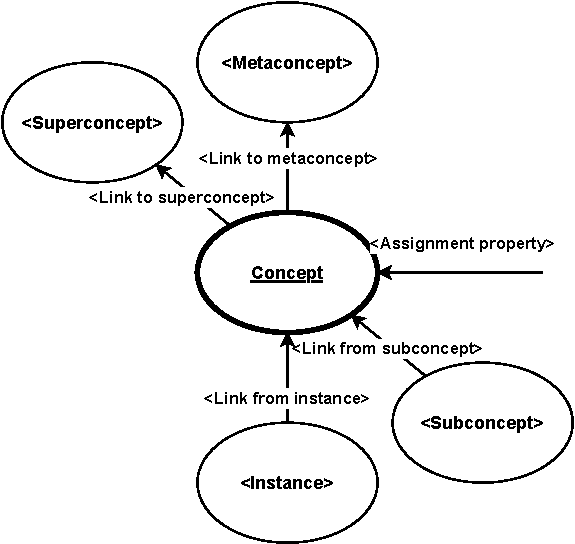
\includegraphics[width=7cm]{figures/conc_diag_templ.pdf}
\caption{Generic template structure}
\label{fig:conc_diag_templ}
%\vspace{-2mm}
\end{figure}

In this respect, note that assigning a concept as a property value is not quite obvious, neither from the formal point of view (specifically, if the concept is represented as an ontological class and not meta-modeled as an individual, whether a code list or knowledge graph one) nor from the semantic point of view.
    The formal compatibility issue was analyzed in the `Classes as Property Values' W3C note \cite{CPV}, on the example of assigning a book the class Lion as its subject (the assignment property being \emph{dc:subject} from the Dublin Core vocabulary), and later partially solved by \emph{punning} (already mentioned in Section~\label{ss:def_type}) being allowed in OWL 2: the individual assigned by the property and the class share the same IRI, but are distinct in the logical space.
The semantic part of the issue was later scrutinized in a study \cite{KCap13} yielding three\footnote{For practical purposes, their numbering in this paper differs from the order in which they are introduced in the old study \cite{KCap13}.} different semantic motivations for `using a class as a property value', yielding three variants (V1--V3) depending on what aspect of the concept is actually to be valued by the property: 
\begin{itemize}
    \item \textbf{V1} the \emph{intension} of the concept, i.e., truly the concept as such;
    \item \textbf{V2} the \emph{extension} of the concept, i.e., the (sub)set of its instances (say, the set of all lions, some particular named lions, or a `prototypical' lion, in the book subject example);
    \item \textbf{V3}  an abstract \emph{topic} (being not a `canonical' universal, as its instantiation is an arguable matter) merely derived from the concept; e.g., a book has as subject the topic of lions rather than the concept of a lion.
    \end{itemize}
Looking at the first variant, we can still formulate some likely sub-variants for it: 
\begin{itemize}
    \item \textbf{V1a} The property is a `hooded' \emph{instantiation}, merely expressed by a custom property -- say, \emph{ex:speciesOfExemplar} (assigning an animal to its species or another taxon), if we stick to the class Lion as property value -- than by \emph{rdf:type}. Such a property is then not truly an assignment property but provides linking from instances, with respect to our template structure.
    \item \textbf{V1b} The property is, in a way, an inverted meta-property of the concept -- e.g., \emph{ex:proposedAsTaxon}, linking a biologist to their invented and proposed taxa, in the biological setting (some less ancient taxon than Lion should probably be used as a real example here). 
\end{itemize}

Let us now go through the expected ways the template is instantiated with respect to our three different types of knowledge representation.
For each of them we characterize the expected template instantiation (i.e., what kind of entities is likely to appear in the context of an entity representing a concept) for each of the knowledge representations, in a table (Table~\ref{tab:comparison}), also showing an example diagram using the same layout as in the template diagram. 
Aside the structural context, we could also consider other aspects of the concept representation and management. 
Here we consider one complex aspect, the maintenance of the concept, in time, characterized in the last row of Table~\ref{tab:comparison}.



\subsection{Concept as an OWL class}

Modeling a concept as a class is the approach in which the logical semantics interweaves most closely with the deeper ontological semantics.
The only meta-concept of a class is normally (under the DL semantics) the specific \emph{rdfs:Class} entity (sometimes non-canonically substituted by \emph{owl:Class}).
Linking from instances via \emph{rdf:type}, and to super-concepts and from sub-concepts via \emph{rdfs:subClassOf}, is quite an obvious option.
On the other hand, as explained in Section~\ref{ss:template}, the use of assignment properties is trickier and has to rely on punning.
As designers of ontologies meant for real adoption will likely not obscure them with punning, the assignment properties, if any, would probably belong to a separate namespace. 

As an example, see the class \emph{dbo:Stream}, from the DBpedia Ontology, in Figure~\ref{fig:conc_diag_class}. 
The diagram contains elements of the real context of this class in the ontology and instance knowledge graph.
The only exception is the artificially added assignment property \emph{ex:hasHabitat}, thus displayed in grey.
It is an example of the variant V2 from Section~\ref{ss:template}: some animal, say, fish, lives in particular (certainly not even all) instances of stream, and not in the `stream concept' itself.


\begin{figure}[h]
\centering
%\captionsetup{justification=centering}
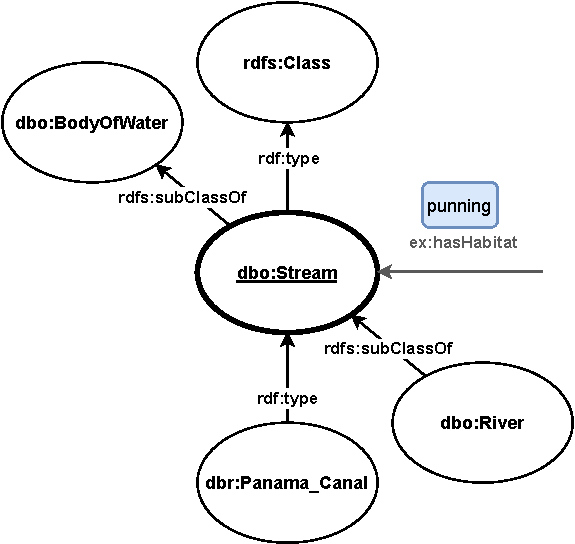
\includegraphics[width=7cm]{figures/conc_diag_class.pdf}
\caption{Class instance example from DBpedia}
\label{fig:conc_diag_class}
%\vspace{-2mm}
\end{figure}

As regards the maintenance of a class within an ontology, its complete replacement by another one is not common, since the curator of the ontology usually has no control on what and how many datasets already link to it; even if there is a new class with an altered definition, the old class is kept with an equivalence link to the new one (and with a `Deprecated' annotation label).
Furthermore, even if there may be closely related sets of sibling (or parent/child) classes, often such an update is applied on them individually.

%\medskip
%As we saw, there are many variations and subtle nuances of why and how concepts are modeled and linked in RDF knowledge bases.
%In the rest of the paper we will however confine ourselves to the situation from Figure~\ref{fig:conc_diag_c_ind}, where a code list is embedded in an ontology.


\begin{figure}[h]
\centering
%\captionsetup{justification=centering}
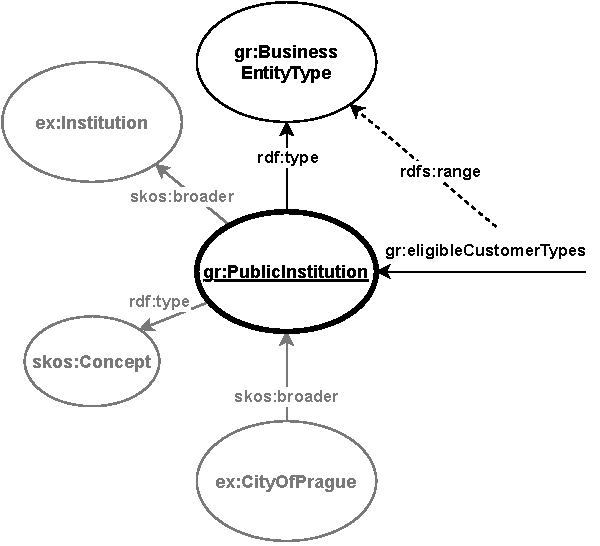
\includegraphics[width=7cm]{figures/conc_diag_c_ind}
\caption{Instance example from the GoodRelations ontology}
\label{fig:conc_diag_c_ind}
%\vspace{-2mm}
\end{figure}

\subsection{Concept as a code list individual}

%While the extraction of code lists in Section~\ref{s:codelistanalyzer} was entirely devoted to code lists embedded in ontologies, we will here review the expected setting covering even more stand-alone code lists, such as those primarily foreseen in the EU guidelines \cite{guide_code_list}.

First of all, the individual representing the concept will usually be linked via \emph{rdf:type} to a domain-specific class -- the \emph{code list class}.
The designers of the ontology often hint on the meta-modeling nature of this class by employing a naming convention: providing it with an ending such as ``-Type'' or ``-Kind''.
SKOS structures may be applied to express the links to super- and sub-concepts (\emph{skos:broader} and  \emph{skos:narrower}).
However, we would not expected to see linked instances: since the concept is modelled in the context of an ontology (within an embedded code list), if the designer wished to instantiated the given concept, s/he would have had the choice to express it as a class rather than as an individual.
The concept itself will then also be additionally typed as \emph{skos:Concept}, and linked to a SKOS concept scheme via \emph{skos:inScheme}.
For embedded code lists, it may typically be the case that they would be designed to serve a single assignment property, from the same namespace.
For standalone code lists with highly reusable codes (such as legal forms of organizations, or commodity types), linking via using multiple, independent, assignment properties is quite possible.

The example in Figure~\ref{fig:conc_diag_c_ind} shows the context of the \emph{gr:PublicInstitution} individual from the GoodRelations ontology \cite{GR}.
The individual is one of the four pre-defined individuals of the \emph{gr:BusinessEntityType} class (others are \emph{gr:Business}, \emph{gr:Enduser} and \emph{gr:Reseller}); note the naming pattern present in this (code list) class name.
SKOS is not referred to inside the whole GoodRelations specification; in the diagram, we however demonstrate its possible use (in grey), for better instructiveness.
There is however an assignment property, \emph{gr:eligibleCustomerTypes}.
It is the only property having \emph{gr:BusinessEntityType} as its range.
By the distinctions made in Section~\ref{ss:template}, the assignment of the concept by the property is, again, that of V2: individual public institutions (rather than the notion of a public institution) are eligible for a given business offer.


As regards maintenance, embedded code lists are likely to be updated with their code list classes as wholes, i.e., at irregular times.
Standalone code lists, such as those corresponding to RDF versions of official code lists used by government authorities \cite{DBLP:conf/smap/FilippidisKKIB16}, may, in turn be updated regularly, e.g., annually.

\subsection{Concept as a knowledge graph individual}

Knowledge graphs are typically very large structures, powered by extractions from documents and/or large-scale crowdsourcing.
They have natural propensity to modeling primarily via individuals, as it makes the graph simpler to handle.
These individuals are, in turn, secondarily endowed with links to classes from (typically, multiple) ontologies.
SKOS structures may sometimes be applied, namely, for portions of knowledge graphs that are inherently of hierarchical nature, such as category systems of underlying textual resources (the category system of Wikipedia, transferred to DBpedia, is a prominent example).
Knowledge graph concepts may have multiple independently created links to/from various context elements (in the sense of our framework).
As regards concept maintenance, individual knowledge graph concepts and links between them may often be updated in isolation, in arbitrary times (or, in knowledge graphs derived from textual resources such as Wikipedia, in arbitrary builds applied on these textual resources).

As a first example, in Figure~\ref{fig:conc_diag_kg_ind1}, we see the context of the \emph{dbc:Torpedo\_boats} individual from the DBpedia knowledge graph.
This individual is derived from the corresponding Wikipedia category.
Note that while the link from a sub-concept and that to the super-concept are defined via \emph{skos:broader}, the link from an instance and that to the super-class are defined via \emph{dct:subject}: a property that would not naturally be perceived as an analog of \emph{rdf:type} in the instance-to-instance setting.  
As the modeling derived from Wikipedia categories is inherently hierarchical, there are no properties that could be interpreted as assignment properties in terms of our framework.

\begin{figure}[h]
\centering
%\captionsetup{justification=centering}
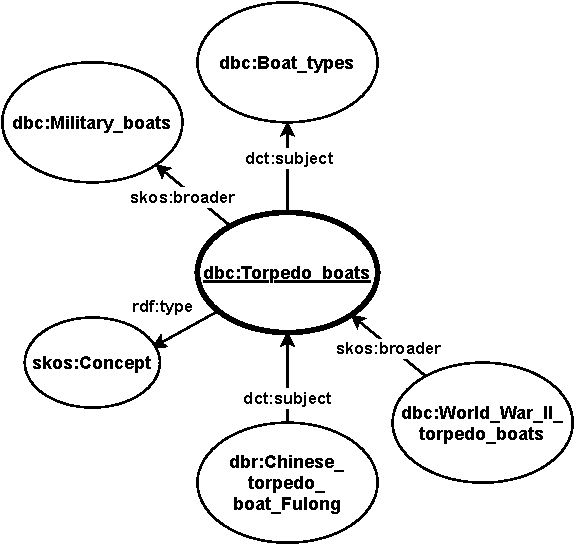
\includegraphics[width=7cm]{figures/conc_diag_kg_ind1.pdf}
\caption{Instance example from DBpedia}
\label{fig:conc_diag_kg_ind1}
%\vspace{-2mm}
\end{figure}

The second example, while also from DBpedia, is structurally completely different. 
In Figure~\ref{fig:conc_diag_kg_ind2} we see the context of the \emph{dbr:Wolverine} individual, which is a common resource derived from a Wikipedia page.
Note that \emph{rdf:type} is used here for the links both to a meta-concept and to a super-concept. 
This illustrates the common assumption that ontological cleanness is not always catered for in knowledge graphs.
As examples of assignment properties applied with the given concept, we show two.
If we look at them from the point of view of the distinctions from Section~\ref{ss:template}, the assignment of the concept by the property \emph{dbp:mascot} is likely a special kind of V2: the wolverine assigned (e.g., to some school) as mascot is not a real animal but a prototype one, yet, it is natural to view it as an instance of the wolverine concept.
The second property, \emph{dbp:shipNameSake}, in turn, rather falls under V1: if the \emph{name} of a ship is derived from the name of the biological genus, the assignment rather targets the intension of the concept.

\begin{figure}[ht]
\centering
%\captionsetup{justification=centering}
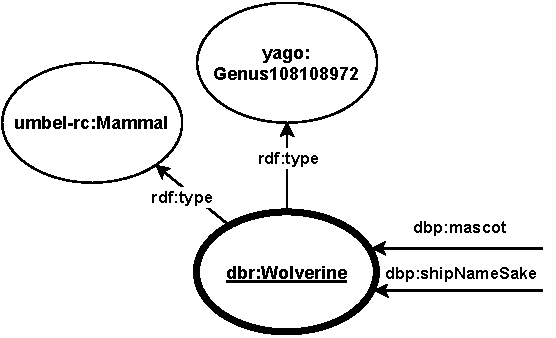
\includegraphics[width=7cm]{figures/conc_diag_kg_ind2.pdf}
\caption{Instance example from DBpedia with assignment properties}
\label{fig:conc_diag_kg_ind2}
%\vspace{-2mm}
\end{figure}







\section{Dimensional analysis of individuals in ontologies}
% pův.: Analysis of code list modeling practice
\label{s:analysis_code_list_modeling_practice}

As we discussed in the previous section, the appearance of individuals in ontologies may indicate that the designers wished to refer to domain-relevant concepts without having to express them via classes (and at the same time did not want to hold them in a separate instance-level knowledge graph).
However, the syntactic status of an ontology-embedded individual might not necessarily be a guarantee of its relevance for a code list. 
In Section~\ref{ss:def_patt} we already mentioned multiple potential reasons for introducing individuals in ontologies, with varying degree of relevance for the code list setting.
The queries from Section~\ref{s:codelistanalyzer}, implemented in Code List Analyzer, were driven by heuristics on what \emph{is} a candidate code list structure, and allowed to manually inspect the \emph{precision} of these heuristics.
However, the cases not corresponding to those heuristics, were not retrieved; the presence of false negatives in the queries might then lead to worsened \emph{recall}. 
Since the overall amount of individuals detected in ontologies is not overwhelming, we decided to proceed to their exhaustive analysis, using a dimensional model in which their distribution can be well visualized.
This way, the adequacy of the current Code List Analyzer queries can be, to some degree, evaluated. 

%Apart from verifying the results of the code list extraction as such, we were also interested in uncovering the state-of-the-art styles of modeling embedded code lists inside ontologies and vocabularies. To achieve this, 
Technically, we took a bottom-up approach by querying for a list of all instances from the LOV database dump of 818 vocabularies. The results show that only 229 
vocabularies have at least one class instance embedded inside. The goal of this analysis is to find out in which case the code structures that were identified could or could not count as code lists from the point of view of the meanings of the codes. To assess each code, we have defined and used three determinative binary dimensions by asking the following questions: %1) Is the instance an instance of a class defined in its ontology? 2) Is the instance modeled per SKOS? 3) Is the instance part of the ontology namespace?

\begin{enumerate}
    \item Is the instance an instance of a class defined in its ontology?
    \item Is the instance modeled using SKOS?
    \item Is the instance part of the ontology namespace?
\end{enumerate}

To help answer these questions, the following attributes were identified to be included in the data for our analysis:

\begin{flushleft}
\begin{enumerate}
    \item the class which the instance instantiates,
    \item whether the instance is an instance of a \textit{skos:Concept},
    \item whether the instance is part of a \textit{skos:ConceptScheme} via the property \textit{skos:inScheme},
    \item the namespace of the ontology in which the instance is defined, and
    \item the namespace taken from the IRI of the instance.
\end{enumerate}
\end{flushleft}

To know whether an instance belongs to the ontology's namespace we simply compare these namespaces with the namespaces of the instances that we derived from their IRI. %Table \ref{tab:manual-analysis} shows an excerpt of the retrieved data for our analysis.

\begin{table*}[ht]
\footnotesize
\centering
\begin{tabular}{llll}
\hline
\multicolumn{1}{|l|}{\textbf{instance}} & \multicolumn{1}{l|}{\textbf{class}}                   & \multicolumn{1}{l|}{\textbf{skosConcept}} & \multicolumn{1}{l|}{\textbf{skosConceptScheme}} \\ \hline
geop:AMU                                & geop:economic\_region                                 & -                                         & -                                               \\
gr:Business                             & gr:BusinessEntityType                                 & -                                         & -                                               \\
pproc:AdministrativeInformation         & -                                                     & skos:Concept                              & pproc:InformationKindScheme                     \\
pc:Negotiated                           & -                                                     & skos:Concept                              & -                                               \\ \hline
\multicolumn{1}{|l|}{\textbf{instance}} & \multicolumn{1}{l|}{\textbf{ontology vann:namespace}} & \multicolumn{2}{l|}{\textbf{instance namespace}}                                            \\ \hline
geop:AMU                                & http://aims.fao.org/aos/geopolitical.owl\#            & \multicolumn{2}{l}{http://aims.fao.org/aos/geopolitical.owl\#}                              \\
gr:Business                             & http://purl.org/goodrelations/v1\#                    & \multicolumn{2}{l}{http://purl.org/goodrelations/v1\#}                                      \\
pproc:AdministrativeInformation         & http://contsem.unizar.es/def/sector-publico/pproc\#   & \multicolumn{2}{l}{http://contsem.unizar.es/def/sector-publico/pproc\#}                     \\
\textit{pc:Negotiated}                  & \textit{http://contsem.unizar.es/def/sector-publico/pproc\#}   & \multicolumn{2}{l}{\textit{http://purl.org/procurement/public-contracts\#}}                         
\end{tabular}
\caption{Multi-dimensional analysis data examples, generated by our custom SPARQL-based script %\cref{note:customScript} 
(\textit{on the last row is an example where the ontology namespace does not equal the instance namespace})}
\label{tab:manual-analysis}
\end{table*}

The algorithm for retrieving all relevant data is straightforward. First, we run a query (Code listing \ref{lst:sparql11}) to get a list of all vocabularies and their namespaces in LOV:

\begin{lstlisting}[captionpos=b, caption=Query to retrieve all ontologies and their namespaces,label=lst:sparql11,basicstyle=\ttfamily,frame=single]
SELECT * WHERE {
  ?o a owl:Ontology .
  OPTIONAL { 
    ?o vann:preferredNamespaceUri ?ns . 
  }
}
\end{lstlisting}

And then for each ontology we have a query (Code listing \ref{lst:sparql11}) to find class instances and entities, which are part of a \textit{skos:ConceptScheme}:

\begin{lstlisting}[captionpos=b, caption=Query to retrieve all class instances and skos:ConceptScheme members,label=lst:sparql12,basicstyle=\ttfamily,frame=single]
SELECT DISTINCT ?i
FROM <${ontology}>
WHERE {
 {
  VALUES ?class { owl:Class rdfs:Class }
  ?c a ?class .
  ?i a ?c .
 }
 UNION {
  ?i skos:inScheme ?s .
 }
}
\end{lstlisting}

Next, we query for the rest of the predefined attributes for each instance using the query in Code listing \ref{lst:sparql13}, where several generic meta classes are ignored:

\begin{lstlisting}[captionpos=b, caption=Query to retrieve all class instances and skos:ConceptScheme members,label=lst:sparql13,basicstyle=\ttfamily,frame=single]
SELECT DISTINCT ?c ?s
FROM <${ontology}>
WHERE {
 {
  <${instance}> a ?c .
  FILTER(?c NOT IN (
   owl:Class, rdfs:Class,
   owl:DeprecatedClass, owl:Thing, 
   owl:ObjectProperty, owl:OntologyProperty,
   owl:DatatypeProperty, owl:NamedIndividual,
   owl:AnnotationProperty, owl:Ontology,
   rdfs:Resource, rdfs:Datatype,
   rdf:Property, voaf:Vocabulary, 
   skos:ConceptScheme
  ))
 }
 UNION { <${instance}> skos:inScheme ?s . }
}
\end{lstlisting}

Finally, in a script, %\footnote{\label{note:customScript}\url{https://github.com/nvbach91/iga-hybrid/blob/master/cube-analysis/app.js}} 
we implement these queries and consolidate the result data to a final table %\footnote{\url{https://github.com/nvbach91/iga-hybrid/tree/master/cube-analysis/results}} 
(examples in Table \ref{tab:manual-analysis}) which can be used to inspect the instances with all necessary attributes. This script also takes care of computing derived values (such as the column that contains the instance namespaces) for evaluation purposes and analysis. We expect to incorporate the aspect of comparing ontology namespace and instance namespace to our extraction query sequence in Section \ref{s:codelistanalyzer}. This additional information, as one of the results of the dimensional analysis, would help to better decide whether a particular candidate code list is in fact a code list during the querying and evaluation process.


Using the querying procedure above, we have retrieved a total of 21102 instances together with these attributes and aggregated them into the analysis dimensions in Figure \ref{fig:cube-aggregation} where we also show the number of instances in each case where the highest number of instances 11198 belongs to the case \textit{has a class}, \textit{is not SKOS} and \textit{is in ontology namespace}. The data and the code to reproduce these results can be found once more in our GitHub repository\footnote{\url{https://github.com/nvbach91/iga-hybrid/tree/master/cube-analysis} (includes scripts to reproduce results)}.

\begin{figure}[ht]
    \centering
    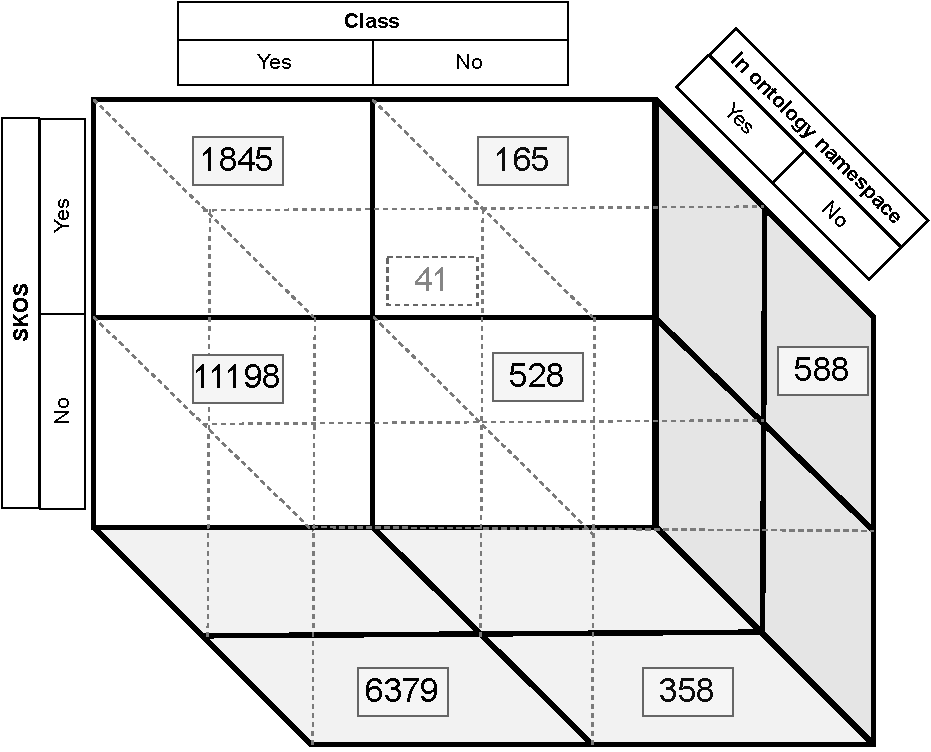
\includegraphics[width=8cm]{figures/cube-aggregation.pdf}
    \caption{Aggregation of instances in three analytical dimensions}
    \label{fig:cube-aggregation}
\end{figure}


\section{Discussion}
\label{s:discussion}
From the aggregation cube in Figure \ref{fig:cube-aggregation} we can see that there are 8 cases to be considered in our analysis. The goal here is to analyze all cases and find out patterns that could represent the characteristics of a code list, whether the instances are (not) part of a code list, why (not), and whether they could be considered as code list members even though they do not have the defining characteristics.

We have found that if an instance is a \textit{skos:Concept} and part of a \textit{skos:ConceptScheme} then it is by definition a code list member and the \textit{skos:ConceptScheme} is the code list, regardless of whether they have a class or not. There are, however, several cases, e.g., \textit{txn:Status\_Preliminary}, \textit{txn:Status\_Testing}, \textit{txn:TaxonConcept\_Scheme}, \textit{pc:Negotiated}, \textit{pc:Open},  \textit{mil:Cavalry},  \textit{mil:Rank\_Private}, where the instance is a \textit{skos:Concept} but not part of a \textit{skos:ConceptScheme}. These are probably desolate instances that do not belong to a higher categorization but still count as codes, and the last reason is simply the link to \textit{skos:ConceptScheme} is unintentionally missing.

Another observation is regarding the fact that there are instances that have a \textit{skos:ConceptScheme} as their class. These of course are the code lists themselves, but not codes of a code list. 

There are also cases where the \textit{skos:ConceptScheme} and the class have similar naming, e.g., \textit{lawd:Reading} and \textit{lawd:readingScheme}. This could mean that the class being instantiated by the codes may theoretically have the same function as the \textit{skos:ConceptScheme} semantically.

The next case is where the instance has a class but is not modeled entirely using SKOS. There are four types of modeling decisions happening here:
\begin{enumerate}
    \item the class implicitly defines a code list as if it were a \textit{skos:ConceptScheme} while the instances are modeled as \textit{skos:Concept}, examples of this case can be found in the Military ontology, e.g. the class \textit{mil:MilitaryRank} and its instances like \textit{mil:Rank\_Private}, \textit{mil:Rank\_Polkovnik}
    \item the class implicitly (and semantically) defines a code list with its instances enumerating obvious codes without the link to \textit{skos:Concept}, e.g., the classes \textit{geop:geographical\_region}, \textit{keys:Key}, \textit{te:TemporalUnit}, \textit{gr:DayOfWeek}, \textit{rlog:Level}, \textit{pso:PublicationStatus},
    \item the instance is a metadata instance used for an annotation property, in this case, it is highly probable that the class comes from a foreign namespace, e.g. \textit{foaf:Person} for contact info,
    \item the instance is an exemplary instance of a class for showcasing purposes, e.g., \textit{ostop:scotland}, in which case this class should be from the same namespace as the instance.
\end{enumerate}

The last case is when an instance does not have a class nor is modeled as SKOS. These are instances of one of the classes in Code listing \ref{lst:sparql13}, which are not relevant in finding code lists, and therefore are ignored during the querying process.

The multi-dimensional analysis in Section~\ref{s:analysis_code_list_modeling_practice} represented a complementary view on the individuals from LOV vocabularies, with respect to the SPARQL extraction patterns from Section~\ref{s:codelistanalyzer}.
It leads us to also check whether the `negatives' wrt. the queries are true or false negatives, i.e., brought us at least qualitative (and satisfactory) insights related to the recall of these queries: the individuals not covered by the queries do not appear as codes making part of code lists.
%Since the tooling used in the multi-dimensional analysis was not confined to SPARQL, we added the namespace correspondence as a third dimension, which 


%\begin{table}[]
%\footnotesize
%\centering
%\begin{tabular}{|l|l|}
% \hline
%owl:Thing              & skos:ConceptScheme \\ \hline
%owl:Ontology           & voaf:Vocabulary    \\ \hline
%owl:NamedIndividual    & rdf:Property       \\ \hline
%owl:ObjectProperty     & rdfs:Class         \\ \hline
%owl:AnnotationProperty & owl:Class          \\ \hline
%owl:DatatypeProperty   & rdfs:Datatype      \\ \hline
%owl:OntologyProperty   & rdfs:Resource      \\ \hline
%\end{tabular}
%\caption{List of ignored classes}
%\label{tab:ignored classes}
%\end{table}


%1 - skriptem

%2 - multidimenzialne predtim nenapadla (shoda namespace)




\section{Related Research}
\label{s:related}
We are unaware of any research project in the ontology and linked data community aiming at systematically analyzing embedded code lists. 
There have, however, been several partially related projects.

The `value partitions vs. value sets' design pattern by Rector \cite{alanrector}, which we discussed in Section~\ref{s:codelist-def}, analyzed the consequences of using a set of individuals vs. sibling classes for representing pre-defined values of properties.
This was however an educational resource, not accompanied by an empirical study showing how often any of the options are actually used.
Also, the intended usage (assigning individuals to expressions from richly axiomatized ontologies) was slightly different from that foreseen for code lists.

Abdul Manaf et al. \cite{Yati_eswc12} studied a large set of SKOS vocabularies on the web.
They concluded that some vocabularies do not fulfill the expectations of a thesaurus, as they do not have the usual lexical labels (such as \emph{skos:prefLabel}) and may also not contain a hierarchy.
We conjecture that some of those SKOS structures may actually correspond to code lists.
Later on, Abdul Manaf in her thesis also elaborated on the problem of converting OWL hierarchies to SKOS taxonomies \cite{Yati-thesis}; this approach corresponds, to a certain degree, to bridge between two of the approaches we study in our analysis.

A detailed study related to the occurrence and acceptance of SKOS for representing existing knowledge organization systems and exposing them on the Semantic Web was also carried out, with a special focus on social aspects of such an adoption \cite{DBLP:journals/corr/abs-1801-04479}.


The topic of code list extraction was covered by the OpenBudgets.org project \cite{DBLP:conf/icwe/MusyaffaHLOJAV18}, where RDF code lists were extracted automatically, through pipeline-based tools, from non-RDF resources (most often in the CSV format) \cite{DBLP:conf/smap/FilippidisKKIB16}.
Since the core fiscal data processed in the project were modeled according to the Data Cube vocabulary \cite{data_cube}, these code lists were not primarily intended for cross-domain use but rather connected to fiscal data components (dimensions of multi-dimensional data cubes).

As regards the problems related to the interplay of upward and downward links of concepts corresponding to both subsumption and instantiation relationships, which we analyze and illustrate in Section~\ref{s:repr}, they have been thoroughly studied by the authors of the Multi-Level Theory \cite{conf/er/AlmeidaFC17}, as well as in other approaches to multi-level modeling \cite{journals/dagstuhl-reports/AlmeidaFK17}.
Our study is definitely lightweight as regards the study of phenomena arising in the presence of multiple levels in a knowledge base, in general, and focuses on the real-world practice in certain OWL ontologies, code lists, and knowledge graphs.

\section{Conclusions}
\label{s:conclusion}
%The presented approach...
In this paper, we have described our workflow and implementation for the semi-automatic detection, extraction, and analysis of code list structures embedded in OWL ontologies. 
%In this paper, we have showcased our experimental approach and our 
The implementation is primarily based on SPARQL queries.
%for the detection and analysis of code list structures in the chosen knowledge base LOV. 
As input material we chose the collection of ontologies indexed in the LOV catalog.
The tool is freely accessible, and also so is the result of its run on the LOV resource, including all scripts and manuals to reproduce results in future iterations.

%Next, we have discussed the motivation for analyzing each structural part of the RDF knowledge representation including a brief comparison for these structural parts from our point of view.
The design of the queries was informed by a comprehensive analysis of possible patterns that could express the general notion of code list in OWL.
Looking at the semantics of code lists, we identified the phenomenon of individuals frequently representing ontological universals. 
This led us to a contextual, qualitative study of alternative ways the designers can choose to represent concepts (universals).
We consequently focused on code lists represented as sets of syntactic individuals embedded in vocabularies in the LOV database.
Under this optic, we also carried out a complementary bottom-up analysis of all such individuals, quantified their position in a multi-dimensional space of features, and qualitatively analysed the different cases.

%Lastly, we have provided results achieved from our workflow, revealing a comprehensive collection of statistical information involving code list occurrences and their structure in LOV.

%Since the research is a part of a larger effort in studying the interplay of concept modeling in `hybrid' representations, having concepts (universals) as classes, code list individuals and possibly even `knowledge-graph-style' individuals, in a single (though, modular) knowledge base, the introductory part of the paper also provided a broader view of this modeling landscape.

We are aware of limitations of our approach, which we aim to overcome in our future work.
Foremost, while the individuals embedded in ontologies were a relatively easy target, they only represent a fraction of structures potentially usable as stand-alone, SKOS-conformant code lists on the Semantic Web.
We assume that a further wealth of code list structures could be obtained by transformation from classes, and possibly also by extraction from large knowledge graphs. 
This will however require additional patterns to be formulated and tested, and it might be hard to reach satisfactory accuracy.
Furthermore, while we believe that the final result produced by our workflow, namely, a dataset of stand-alone code lists, will find its consumers, we have not yet elaborated techniques by which data and knowledge engineers could be informed about the existence of a code list satisfying their needs. 
The practice of communities that routinely handle code lists (even beyond the Semantic Web), such as librarians or public officers, should be studied in order to offer them a mechanism to retrieve code lists built on the basis of ontologies and knowledge graphs, and this way interconnect them to the Semantic Web effort.

%Our future work will focus on: (1) querying and analyzing additional open knowledge graphs with an available SPARQL endpoints found in SPARQLES \cite{DBLP:journals/semweb/VandenbusscheUM17} or other datasets; (2) the ontological analysis of the meaning of codes, namely how often they correspond to ontological universals or particulars; (3) the lexical analysis of patterns within the embedded code list structure wrt their overarching class and the property they provided values for; (4) and finding the motivations for incorporating code lists into the Semantic Web rather than preserving an ontology-instance knowledge graph dichotomy.

%%
%% The acknowledgments section is defined using the "acks" environment
%% (and NOT an unnumbered section). This ensures the proper
%% identification of the section in the article metadata, and the
%% consistent spelling of the heading.
\section*{Acknowledgement}
This research was supported from the institutional-support fund for long-term conceptual development of science and research at the Faculty of Informatics and Statistics of the Prague University of Economics and Business (IP400040), and by the project IGA V\v{S}E \textnumero\ F4/33/2019.




%%
%% The next two lines define the bibliography style to be used, and
%% the bibliography file.
%\bibliographystyle{cas-model2-names} 
%\bibliography{cas-refs}

\bibliographystyle{ieeetr} 
\bibliography{cas-refs}

%%
%% If your work has an appendix, this is the place to put it.
%\appendix

%\section{Research Methods}
 

\end{document}

\endinput
